\documentclass[journal,comsoc]{IEEEtran}
\usepackage[T1]{fontenc}
\usepackage{amsmath}
\interdisplaylinepenalty=2500
\usepackage[cmintegrals]{newtxmath}
\usepackage[numbers,sort&compress]{natbib}
\bibliographystyle{IEEEtran}
\usepackage{graphicx}
\usepackage{epsfig}
\usepackage{CJK}
\usepackage{amsmath}
\usepackage{multirow}
\usepackage{subfigure}
\begin{document}
\title{Dense Network with Correlated Shadow Fading}
%
%
% author names and IEEE memberships
% note positions of commas and nonbreaking spaces ( ~ ) LaTeX will not break
% a structure at a ~ so this keeps an author's name from being broken across
% two lines.
% use \thanks{} to gain access to the first footnote area
% a separate \thanks must be used for each paragraph as LaTeX2e's \thanks
% was not built to handle multiple paragraphs
%




\author{Tingting~Lu,~\IEEEmembership{Student Member,~IEEE,}
        Pei~Liu,~\IEEEmembership{Memver,~IEEE,}
        and~Shivendra~S.~Panwr,~\IEEEmembership{Life~Fellow,~IEEE}% <-this % stops a space
\thanks{T. Lu was with the Department
of Electrical and Computer Engineering, New York University, New York,
NY, 11201 USA e-mail: (tl984@nyu.edu).}% <-this % stops a space
\thanks{J. Doe and J. Doe are with Anonymous University.}% <-this % stops a space
\thanks{Manuscript received April 19, 2005; revised August 26, 2015.}}

\markboth{Journal of \LaTeX\ Class Files,~Vol.~14, No.~8, August~2015}%
{Shell \MakeLowercase{\textit{et al.}}: Bare Demo of IEEEtran.cls for IEEE Communications Society Journals}
\maketitle
\begin{abstract}
In a cellular network, connections between the Base Station (BS) and Mobile Users (MUs) may fail when the channel is in deep fade. Shadow fading is large-scale fading which can cause significant received power loss for a wide area. Correlated shadow fading will result in correlated long outage durations. Power outage will lead to connection loss and/or packet loss which is harmful to MUs, especially to those who are using real-time applications such as video conferencing. Intuitively, increasing BS density is considered to be an efficient way to reduce outage and provide better Quality of Service (QoS) support for delay sensitive applications in noise-limited regime. This paper focuses on a study of the performance of a multi-cell communication system under correlated shadow fading. We consider the downlink direction in a multi-cell communication system. To investigate the outage probability given correlated shadow fading and different BS densities, two system layouts, Grid model and Random model, are studied. First, we compared the outage probability given correlated shadow fading of the two models. The received signal-to-interference-plus-noise ratio (SINR) is calculated. Simulation results show that Grid model outperforms Random model. Secondly, outage probability of Random model with different BS densities are studied. Simulation results suggest that if de-correlation distance is large, increasing BS densities will decrease outage probability. At last, outage durations are investigated to show that higher BS densities will result in shorter outage durations.
\end{abstract}


\begin{IEEEkeywords}
Correlated shadow fading, outage probability, outage duration.
\end{IEEEkeywords}


\section{Introduction and Related Works}

\par In a cellular communication system, the connection between the Base Station (BS) and a Mobile User (MU) may be dropped when the user enters a deep fading area. Fading phenomena can substantially affect the performance of a wireless communication system. In general, fading can be divided into two categories: large-scale fading and small-scale fading. A signal transmitted from source to destination will experience both large-scale and small-scale fading. Small-scale fading is caused by multipath propagation. Large-scale fading, which is also known as shadow fading, is caused by obstacles (trees, buildings, etc.) in the propagation path. In most cases, shadow fading is assumed to be temporally and spatially independent \cite{rappaport1996wireless}.  However, researchers have also shown that shadow fading is spatially correlated at different positions on the propagation path \cite{gudmundson1991correlation}, \cite{zhang2008novel}. In \cite{fabbri2009impact} and \cite{patwari2008effects}, the effects of correlated shadowing in connectivity is demonstrated, which indicates that reliable connectivity will be much more difficult to maintain than indicated by independent shadow fading models. The spatial correlation of shadow fading is important when studying the quality of service of a mobile system since it will result in long-lasting outage durations, which will deteriorate the performance of the applications running on the network. For example, in Figure \ref{building}, the MU is moving behind a row of tall buildings which block the signals from the base station. These tall buildings result in deep shadow fading, and the shadow fading of different positions behind these buildings are closely correlated. To investigate the system performance under correlated shadow fading, this paper focuses on outage probability and outage duration analysis under correlated shadow fading in a multi-cell communication system. Based on the analysis, we provide a solution to reduce the frequency and duration of dropped connections.
\par There have been a lot of studies on the outage probability of cellular communication systems \cite{abu1991outage, petrovic2013outage, emamian2014outage}. The author of \cite{vural2015effect} analyzed the outage probability and coverage area under different independent identical distributed (\emph{i.i.d.}) shadow fading distributions: Log-normal distribution, Weibull distribution and Gamma distribution. In contrast, there is much less work on the system performance given correlated shadow fading. The outage probability and outage duration given correlated shadow fading is still an open problem. In \cite{lu2015long} and \cite{lu2015shining}, authors studied the outage probability and outage duration of a single-cell communication system under exponentially correlated shadow fading and Distance-Angle correlated shadow fading. \cite{lu2015long} the author showed that for a single-cell model, exponentially correlated shadow fading can be modeled as a Markov Chain Model. Highly correlated shadow fading will result in long-lasting outage durations. In \cite{lu2015shining}, single-cell model given distance-angle correlated shadow fading is studied. The correlated shadow fading leads to correlated outage and long outage durations in a single-cell model. A solution to overcome the correlated shadow fading was proposed: relay cooperative communication. The above two papers are limited to single-cell model. In this paper, we are going to extend the study of correlated shadow fading impact to a multi-cell communication system, and provide a solution to overcome the long-lasting outage duration and improve the system performance.
\begin{figure}
\centering
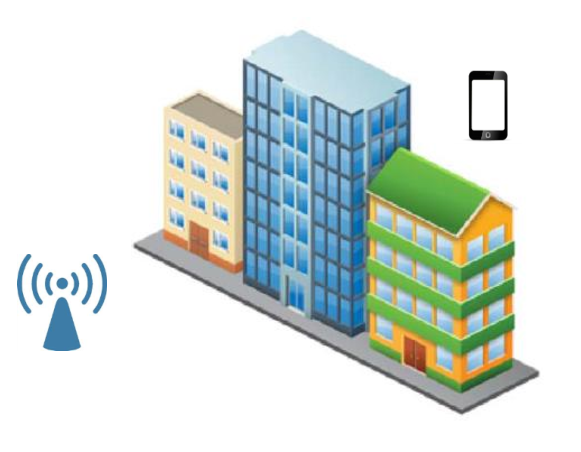
\includegraphics[width=6cm]{building.eps}
\caption{An example of building blockage.}
\label{building}
\end{figure}
\par For multi-cell system, in \cite{andrews2011tractable}, the author developed general models for the multi-cell coverage probability using stochastic geometry. The cellular network is modeled by considering BS locations as a homogeneous Poisson Point Process (PPP). It concluded that under general fading, increasing the number of BSs does not affect the coverage probability (so is the outage probability) while the MU is connected to the nearest BS. The paper also did comparison between grid model and the random PPP model and concludes that  the grid model provides the upper bound of the coverage probability while the PPP provides the lower bound. The author also considered the effect on independent log-normal interference and concludes that the increasing log-normal interference increased the coverage probability, which seems counter-intuitive. Although this paper proposed a general solution to coverage probability, the author didn't consider the scenarios with correlated log-normal shadow fading. The paper focused on coverage probability without investigating the outage duration, which is critical to system performance.
\par In most cases, shadow fading is modeled as an independent log-normal distribution \cite{goldsmith2005wireless} with a standard deviation derived from empirical measurements. An independent log-normal shadowing model is used widely when shadow fading cannot be ignored. In the log-normal shadowing model, the path loss $\psi$ is assumed random, with a log-normal distribution given by
\begin{equation}
p(\psi)=\frac{\xi}{\sqrt{2\pi}\sigma_{\psi_{dB}}\psi}exp[-\frac{(10\log_{10}\psi-\mu_{\psi_{dB}})^{2}}{2\sigma_{\psi_{dB}}^{2}}], \psi>0,
\end{equation}
where $\xi=10/\ln10$, $\mu_{\psi_{dB}}$ is the mean of $\psi_{dB}=10\log_{10}\psi$ and $\sigma_{\psi_{dB}}$ is the standard deviation of $\psi_{dB}$.
The distribution of the $dB$ value of $\psi$ is Gaussian with mean $\mu_{\psi_{dB}}$, standard deviation $\sigma_{\psi_{dB}}$ and is given by:
\begin{equation}
p(\psi_{dB})=\frac{1}{\sqrt{2\pi}\sigma_{\psi_{dB}}}exp[-\frac{(\psi_{dB}-\mu_{\psi_{dB})^2}}{2\sigma_{\psi_{dB}}^2}].
\end{equation}
The above model fails to capture the spatial correlations in shadow fading. Empirical measurements show that shadowing has significant correlations in realistic scenarios that can affect system performance \cite{graziano1978propagation}. Considering the distribution of obstructions and the speed of the MS, a realistic channel propagation model should incorporate correlated shadow fading.  Szyszkowicz et al. \cite{szyszkowicz2010feasibility} presented a review and analysis of the feasibility of different correlated shadowing models.
\par A comparative study of random and grid topology of small cell network deployment was given in \cite{chen2012small}. In this paper, spatial outage probability and spatial average throughput versus the number of access points of the two different network deployment is studied. But this paper considered independent log-normal interference instead of correlated log-normal fading. Approximate outage probability and capacity for $\kappa-\mu$ shadow fading is studied in \cite{kumar2015approximate}. $\kappa-\mu$ shadow fading includes one-side Gaussian, the Rayleigh, the Nakagami-m, the Rician and so on.


\par This paper contains three major parts: first part describes the correlated shadow fading model that was used and the resulting correlated outage field; second part studies the outage probability of the system given different connection strategies; third part presents the simulation and results. The main contributions of this paper is illustrated as follows:
\begin{itemize}
\item An analysis of the relationship between correlated shadow fading and correlated outage events.
\item Comparison of Grid model and Random model performance.
\item Analyze the performance of the Random system model with different BS density. The performance includes computing outage probability (coverage probability) and the outage durations.
\item Propose a strategy to improve system performance by increasing BS density.
\end{itemize}
The paper is organized as follows: Section \ref{CorrShadowField} presents the correlated shadow fading model that is used in this paper and the resultant correlated outage field. Section \ref{SystemModel} presents the system model with two different BS deployment schema. Section \ref{OutageProb} gives theoretical analysis of outage probability. Section \ref{SimuProb} presents the simulation setup and analyzes the simulation results of different BS deployments and densities. Section \ref{Conclusion} summarizes the paper.

\section{Correlated Shadow Fading}
\label{CorrShadowField}
As stated in the introduction, empirical measurements show that there exist different patterns of correlations between the shadowing. The independent log-normal shadow fading model, while very useful for static MS performance analysis, cannot reflect the correlation of shadow fading between different locations. In this section, we will give a brief introduction of shadow fading models, including the model used in this paper.
In most cases, shadow fading is considered as independent log-normal. But from empirical measurements we can conclude that there exit different correlations between shadow fading factor. There is no single mathematical model which captures all different categories of correlation\cite{szyszkowicz2010feasibility}. In this paper, we use the most commonly used exponentially correlated shadow fading model \cite{szyszkowicz2011interference}. In \cite{szyszkowicz2011interference}, the author states that correlation in shadowing is indispensable for the analysis of interference of large networks. An exponentially correlated shadowing field $S$ with shadow fading factor $s_{i}$ for each position $p_{i}$ has a correlation matrix as below:
\begin{equation}
\mathbf{K}_{N\times N} = [ \sigma_{s}(p_{i})\sigma_{s}(p_{j})\rho(i,j)],
\label{correlationmatrix}
\end{equation}
where $N$ is the length of the shadowing field. Suppose $A$ and $B$ are two neighboring points, the shadow fading (in dB) is $N(0,\sigma^2)$ where $\sigma$ is the standard deviation. The spatial correlation between $s_{A}$ and $s_{B}$ will be given by 
\begin{equation}
\rho_{A,B} = \frac{E[s_{A}s_{B}]}{\sigma^2} =e^{-\frac{d_{A,B}}{d_{0}}}
\end{equation}
where $d_{0}$ is de-correlation distance and  $d_{A, B}$ denotes the distance between $A$ and $B$.
\begin{figure}
\centering
\includegraphics[width = 9cm]{ShadowFieldDeCorr20.jpg}
\caption{Exponentially correlated shadowing field with $d_{0} = 20m$ (the color of the area refers to the normalized standard deviation  which is $S_{i}/\sigma_{s}(i)$)}

\label{shadowingfield}
\end{figure}
Follow the shadowing field generation algorithm, we generate shadowing fields with different  de-correlation distances. A sample correlated shadowing field is shown in Figure \ref{shadowingfield}. In figure \ref{shadowingfield}, deeper color means deeper fading. Deep blue colors are aggregating together to show the pattern of correlation. When MU get into the blue region (deep fading region), it will stay in that region for a certain period of time. Due to this correlation, a MU in deep fading area may experience long-lasting outage duration.

\section{System Model and Correlated Outage Area}
\label{SystemModel}
In this paper, we considered two system models with different BS deployment scheme: Grid model and Random model.
\begin{itemize}
\item Grid Model: $\lambda$ BSs are placed on a grid deterministically.
\item Random Model: $\lambda$ BSs are placed randomly in a fixed area.
\end{itemize}
\begin{figure}
\centering
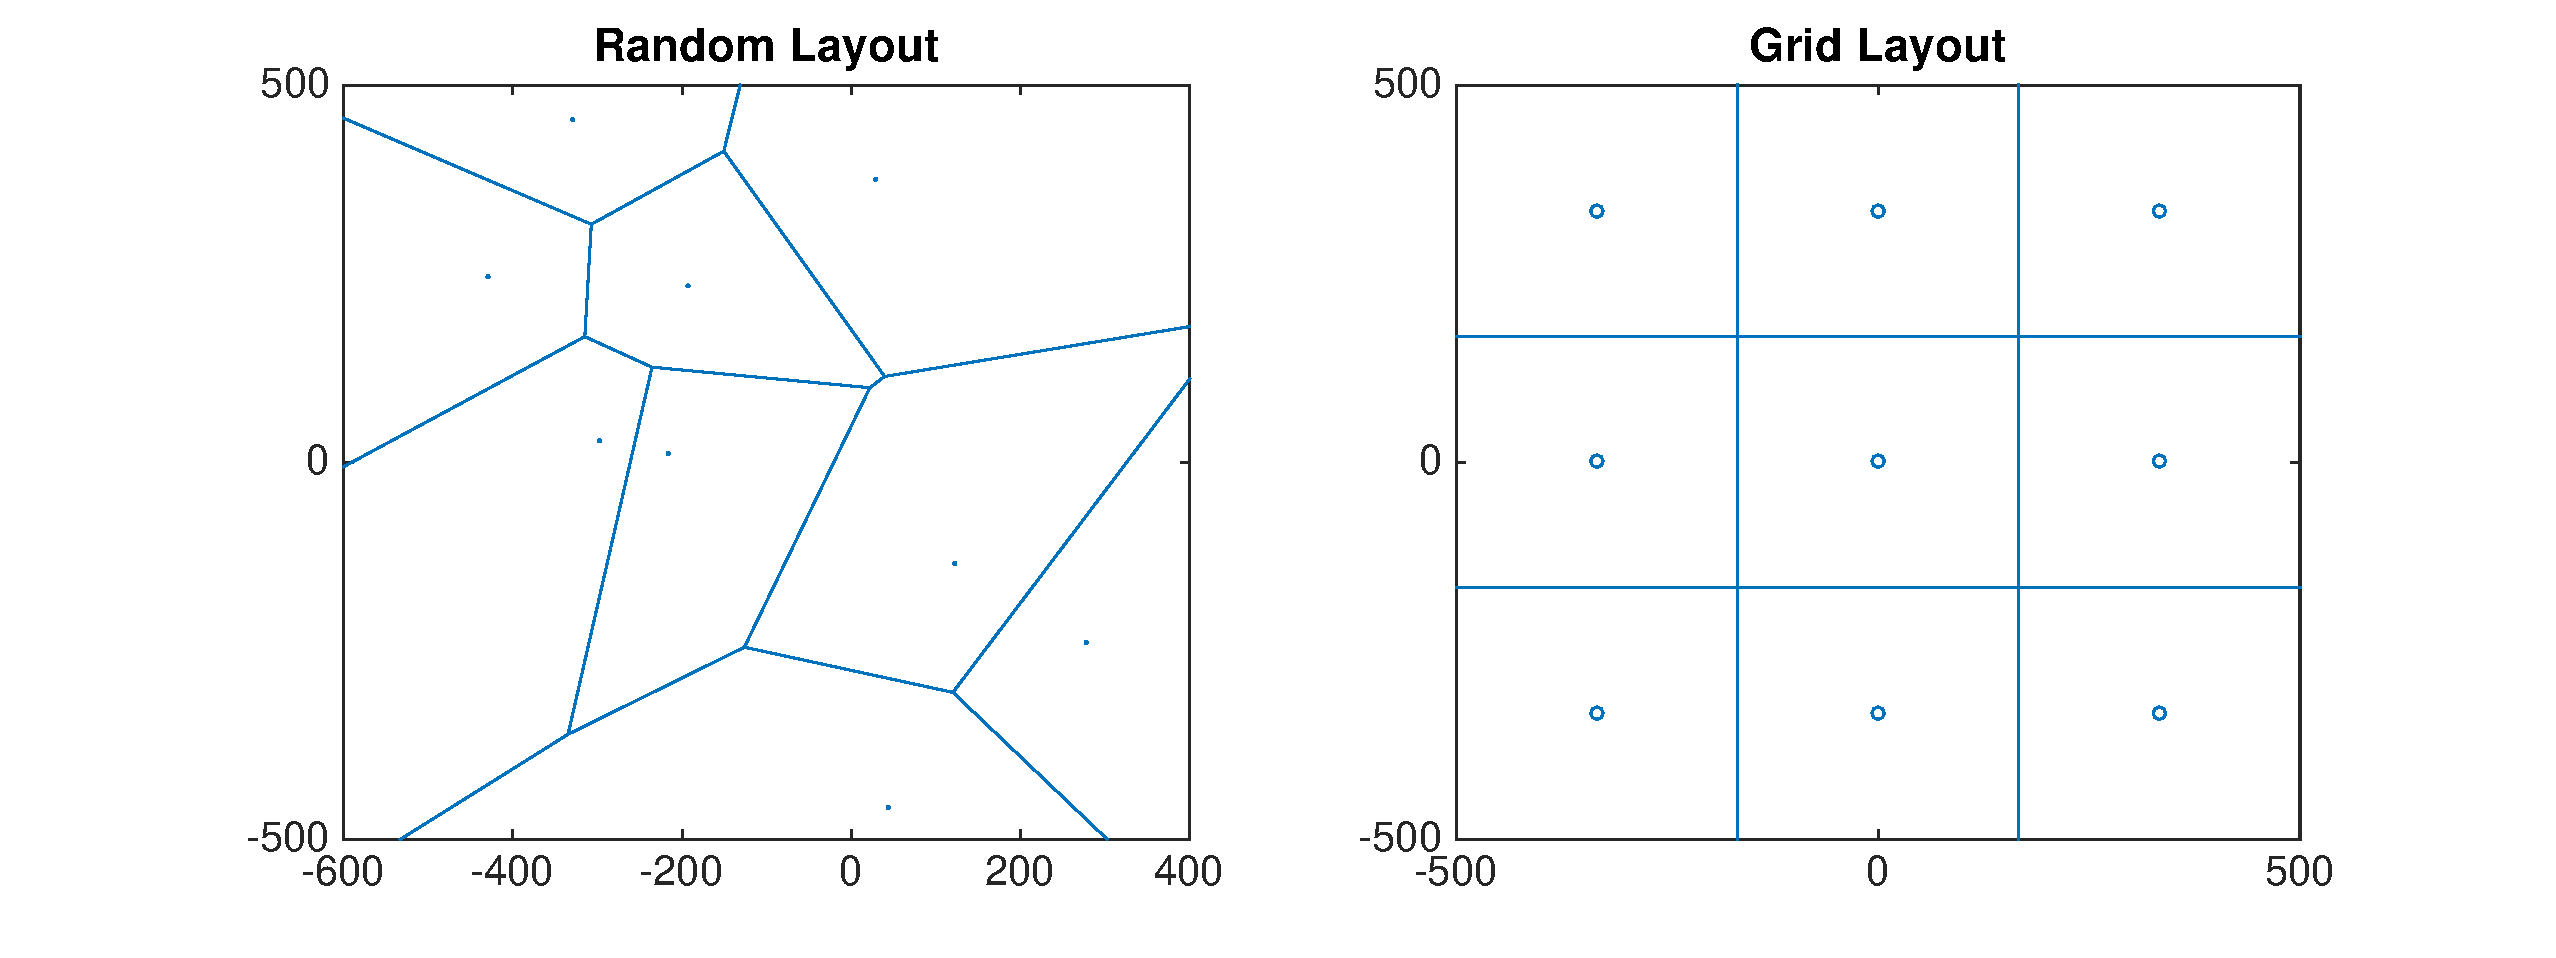
\includegraphics[width=9cm]{systemLayout.eps}
\caption{Random Layout and Grid Layout with $\lambda = 9$.}
\label{RandomLayout}
\end{figure}
% \begin{figure}
% \centering
% \includegraphics[width=8cm]{GridLayout.eps}
% \caption{Grid Base Station Locations}
% \label{GridLayout}
% \end{figure}
Left subfigure of Fig \ref{RandomLayout} is an example of the Grid model, where cells are in regular square shape with same size. For the Random model showed in Fig \ref{RandomLayout} right subfigure, cells are not guaranteed to be the same shape and same size. Distances between different BSs are have a large variation. 
\par Let $\varphi = \{1, 2, \dots, N\}$ denotes the set of all Base Stations, then the received signal from Base Station $j$ to the destination user $D$ is given by:
\begin{equation}
y_{i\to D} = G_{i\to D}x_{i}+n_{D}.
\end{equation}
where $x_{i}$ is the signal transmitted by the source Base Station and $y_{i\to D}$ is the signal received by the destination. $n_{D}\sim \mathcal{CN}(0,N_{0})$ is additive white Gaussian noise. $G_{i\to D}$ is the channel gain from source Base Station to destination including path loss and shadow fading. The end-to-end received signal-to-interference-plus-noise ratio $\text{SINR}$ is given as follows:
\begin{equation}
\text{SINR} \triangleq \frac{P_{i}*G_{i\to D}^{2}}{N_{0}+\sum_{j\in \varphi/i}P_{j}*G_{j\to D}^2},
\end{equation}
where $P_{i}$ is the transmitted power of Base Station $i$. The destination successfully receives the signals if no outage event happens, i.e., $\log_{2}(1+\text{SINR})\ge R$, where $R$ is the required data rate. From the definition of SINR, no outage event happens as long as $\text{SINR} > \gamma$, where $\gamma = 2^{R}-1$.
\par Given a correlated shadowing field, the outage events at different locations are also correlated. Without considering small-scale fading, the channel gain at different locations are spatially correlated. Given a proper threshold $\gamma$, an outage area is defined as SINR less than $\gamma$. Based on the aforementioned correlated shadow fading model and Random system model, a correlated outage filed can be generated as in Figure \ref{outagefie}. On the left, a correlated outage field with independent log-normal shadow fading is shown while the correlated outage field with correlated shadow fading is given on the right. The black color indicates outage areas. Outage area with \emph{i.i.d.} shadow fading are nonconsecutive dots while with correlated fading are connected areas. This demonstrates that correlated shadow fading will result in correlated outage areas.

\begin{figure}
\centering
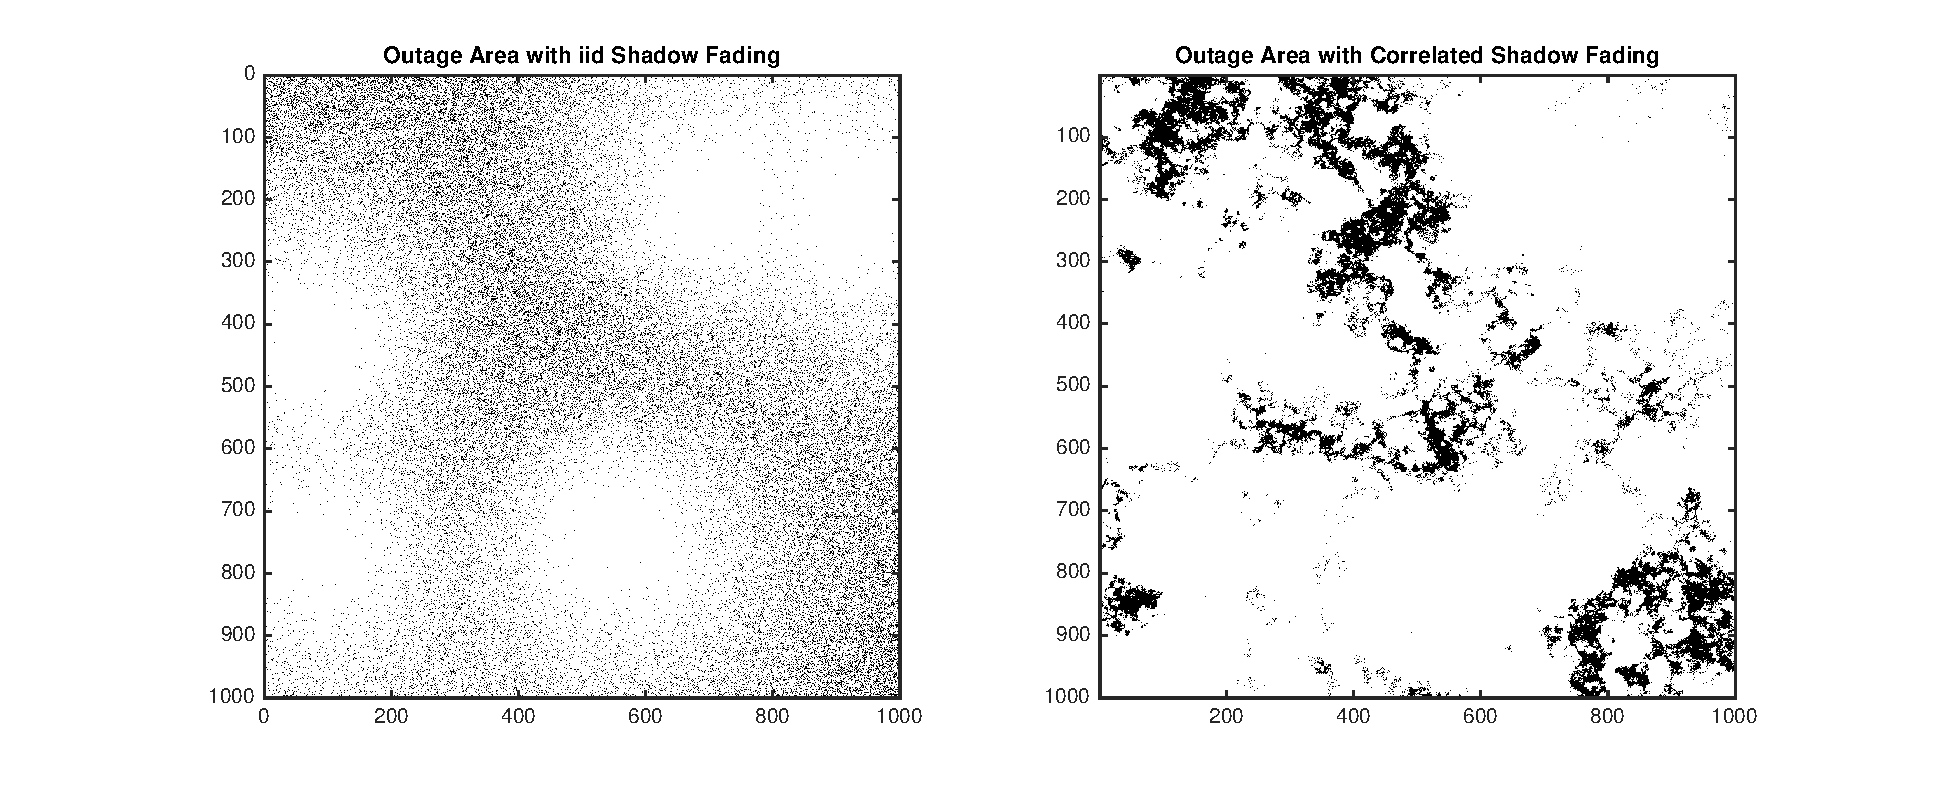
\includegraphics[width=9cm]{outageArea.eps}
\caption{Correlated Outage Fields with $\gamma$ (Dark areas are outage areas while white areas are non-outage areas)}
\label{outagefie}
\end{figure}





\section{Outage Probability Analysis}
\label{OutageProb}
\par For a particular mobile user, outage happens when its received SINR is less than a threshold to decode the received signal. In our scenario, the probability that the receiver cannot decode signals received from its serving Base Station is defined as:
\begin{equation}
P(out_{i}) = P[\text{SINR}_{i\to D} < \gamma],
\end{equation}
Two different connection strategies are discussed in the following sections:
\begin{itemize}
\item: Nearest BS: MU connecting to the BS that is nearest to the MU.
\item Strongest BS: MU connecting to the BS that provides strongest signal to the MU.
\end{itemize}
\begin{figure}
\centering
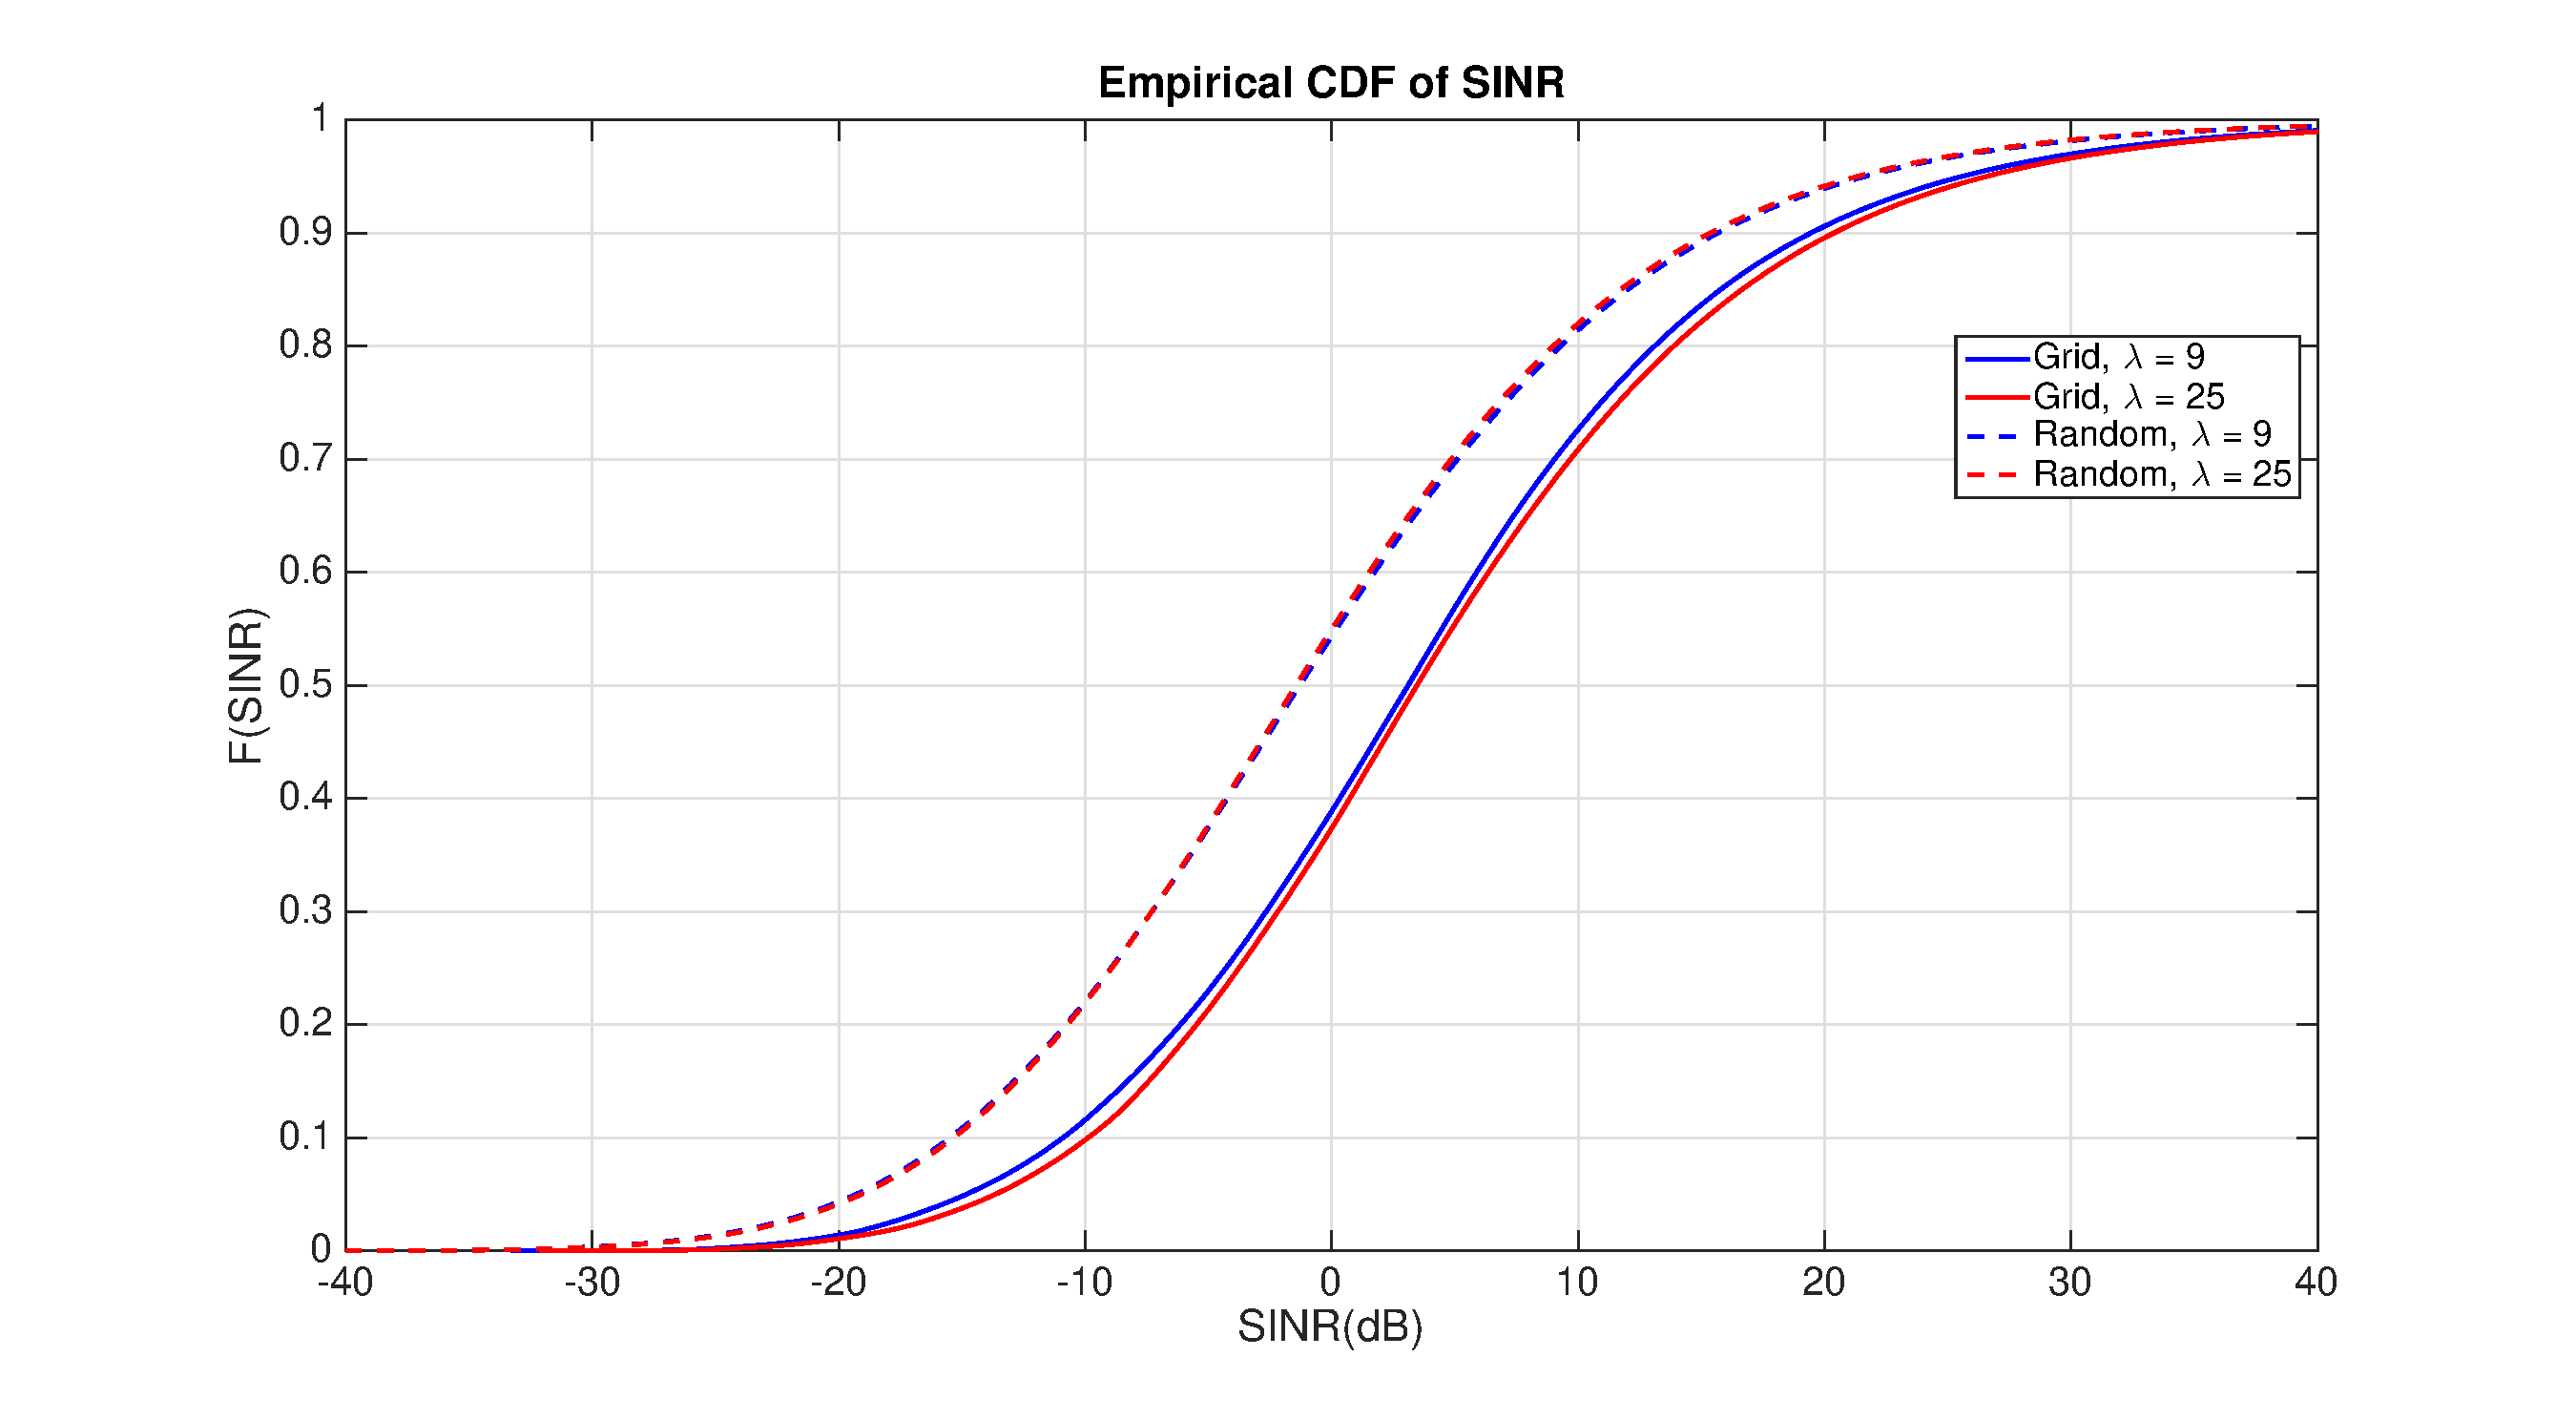
\includegraphics[width=6cm]{GridVSRandom.eps}
\caption{CDF of SINR given Grid Layout and Random Layout (De-Correlation Distance: $20m$)}
\label{cdf1}
\end{figure}
\begin{figure}
\centering
\includegraphics[width=6cm]{OutageProbGridVSRandom.eps}
\caption{Outage Probability given Grid Layout and Random Layout (De-Correlation Distance: $20m$)}
\label{outage1}
\end{figure}
If the MU is serving by the nearest BS, then the outage probability will be $P_{out} = P_{out_{i}}$ where $i$ is the index of the nearest Base Station. If the MU is serving by the BS that provides the strongest signal, the indices of all Base Stations which are able to provide successfully connection to the Mobile User form a set $\mathcal{R}_{n}$. Under the assumption that an MS always connecting to the Base Station which provides the best received signal, the outage event happens if no Base Station can provide big enough SINR to the receiver, which means $\mathcal{R}_{0}=\phi$. Based on this assumption we have:
\begin{equation}
P_{out} = \max_{i = 1,\cdots,N} P[\text{SINR}_{i\to D}<\gamma].
\end{equation}
The probability density function (pdf) of shadow fading $S$ given $L$ correlated fading branches is
\begin{equation}
\begin{split}
f_{\mathbf{S}}(\mathbf{s}) = &\frac{\lambda^{L}}{\sqrt{2\pi}|\mathbf{K}_{L\times L}|^{1/2}\prod_{i=1}^{L}s_{i}}\\
&\cdot\exp(-\frac{1}{2}(10\log_{10}\mathbf{s}-\mathbf{\mu})^{T}\mathbf{K}_{L\times L}^{-1}(10\log_{10}\mathbf{s}-\mathbf{\mu})),
\end{split}
\end{equation}
where $\lambda = 10/\ln10$ and $\mathbf{\mu}$ is the average shadow fading which is normally $0$. $\mathbf{K}_{L\times L}$ is the correlation matrix which is defined in \eqref{correlationmatrix}. Let $\theta_{i} = (10\log_{10}s_{i}-\mu_{i})/\sqrt{2}\sigma_{i}$, and doing a change of variables gives us the pdf of $\mathbf{\Theta}$ as follows:
\begin{equation}
f_{\mathbf{\Theta}}(\mathbf{\theta}) = \frac{1}{\pi^(L/2)|\mathbf{\Sigma}|^{1/2}}\exp(-\mathbf{\Theta}^{T}\mathbf{\Sigma}^{-1}\mathbf{\Theta}),
\end{equation}
where $\mathbf{\Sigma}$ is the correlation coefficient matrix which is
\begin{equation}
\left[\begin{array}{cccc}
1 & h_{1,2} & \cdots & h_{1,L}\\
\vdots & \ddots & \ddots & \vdots\\
h_{L,1} & h_{L,2} & \cdots & 1\\
\end{array}\right].
\end{equation}
Since $\text{SINR}_{i\to D}=PL_{i\to D}+S_{i}-N_{0}-\sum_{j\in\varphi/i}(PL_{j\to D} + S_{j})$ in dB, $\text{SINR}_{i\to D}<\gamma$ means
\begin{equation}
S_{i} - \sum_{j\in\varphi/i}S_{j}<\gamma -PL_{i\to D} + \sum_{j\in\varphi/i}PL_{j\to D} + N_{0},
\end{equation}
Then with the assumption that users are served by the nearest Base Station, the outage probability can be written as:
\begin{equation}
\label{outprob}
P_{out} = \underbrace{\int_{-\infty}^{+\infty}\cdots\int_{-\infty}^{+\infty}}_{i =1,\cdots,N} g(PL_{i}S_{i} - \gamma\sum_{j\in\varphi/i}PL_{j}S_{j})f(\mathbf{s})d\mathbf{s}.
\end{equation}
where $\mathbf{s}$ is the correlated shadow fading experienced by all BSs, $g(PL_{i}S_{i} - \gamma\sum_{j\in\varphi/i}PL_{j}S_{j})$ is a step function defined in (\ref{stepfunction}).
\begin{figure*}[!t]
% ensure that we have normalsize text
\normalsize
% Store the current equation number.
% \setcounter{MYtempeqncnt}{\value{equation}}
% % Set the equation number to one less than the one
% % desired for the first equation here.
% % The value here will have to changed if equations
% % are added or removed prior to the place these
% % equations are referenced in the main text.

\begin{equation}
\label{stepfunction}
g(PL_{i}S_{i} - \gamma\sum_{j\in\varphi/i}PL_{j}S_{j}) = \{\begin{array}{cc}
               1, &  \text{  when }PL_{i}S_{i} - \gamma\sum_{j\in\varphi/i}PL_{j}S_{j} <\frac{\gamma N_{0}}{P}\\
               0, & \text{  when }PL_{i}S_{i} - \gamma\sum_{j\in\varphi/i}PL_{j}S_{j} >\frac{\gamma N_{0}}{P}
             \end{array}.
\end{equation}
% Restore the current equation number.
% \setcounter{equation}{\value{MYtempeqncnt}}
% IEEE uses as a separator
\hrulefill
% The spacer can be tweaked to stop underfull vboxes.
\vspace*{4pt}
\end{figure*}


\section{Simulations and Results}
\label{SimuProb}
\begin{figure*}
\centering
\subfigure[i.i.d. Shadow Fading]{
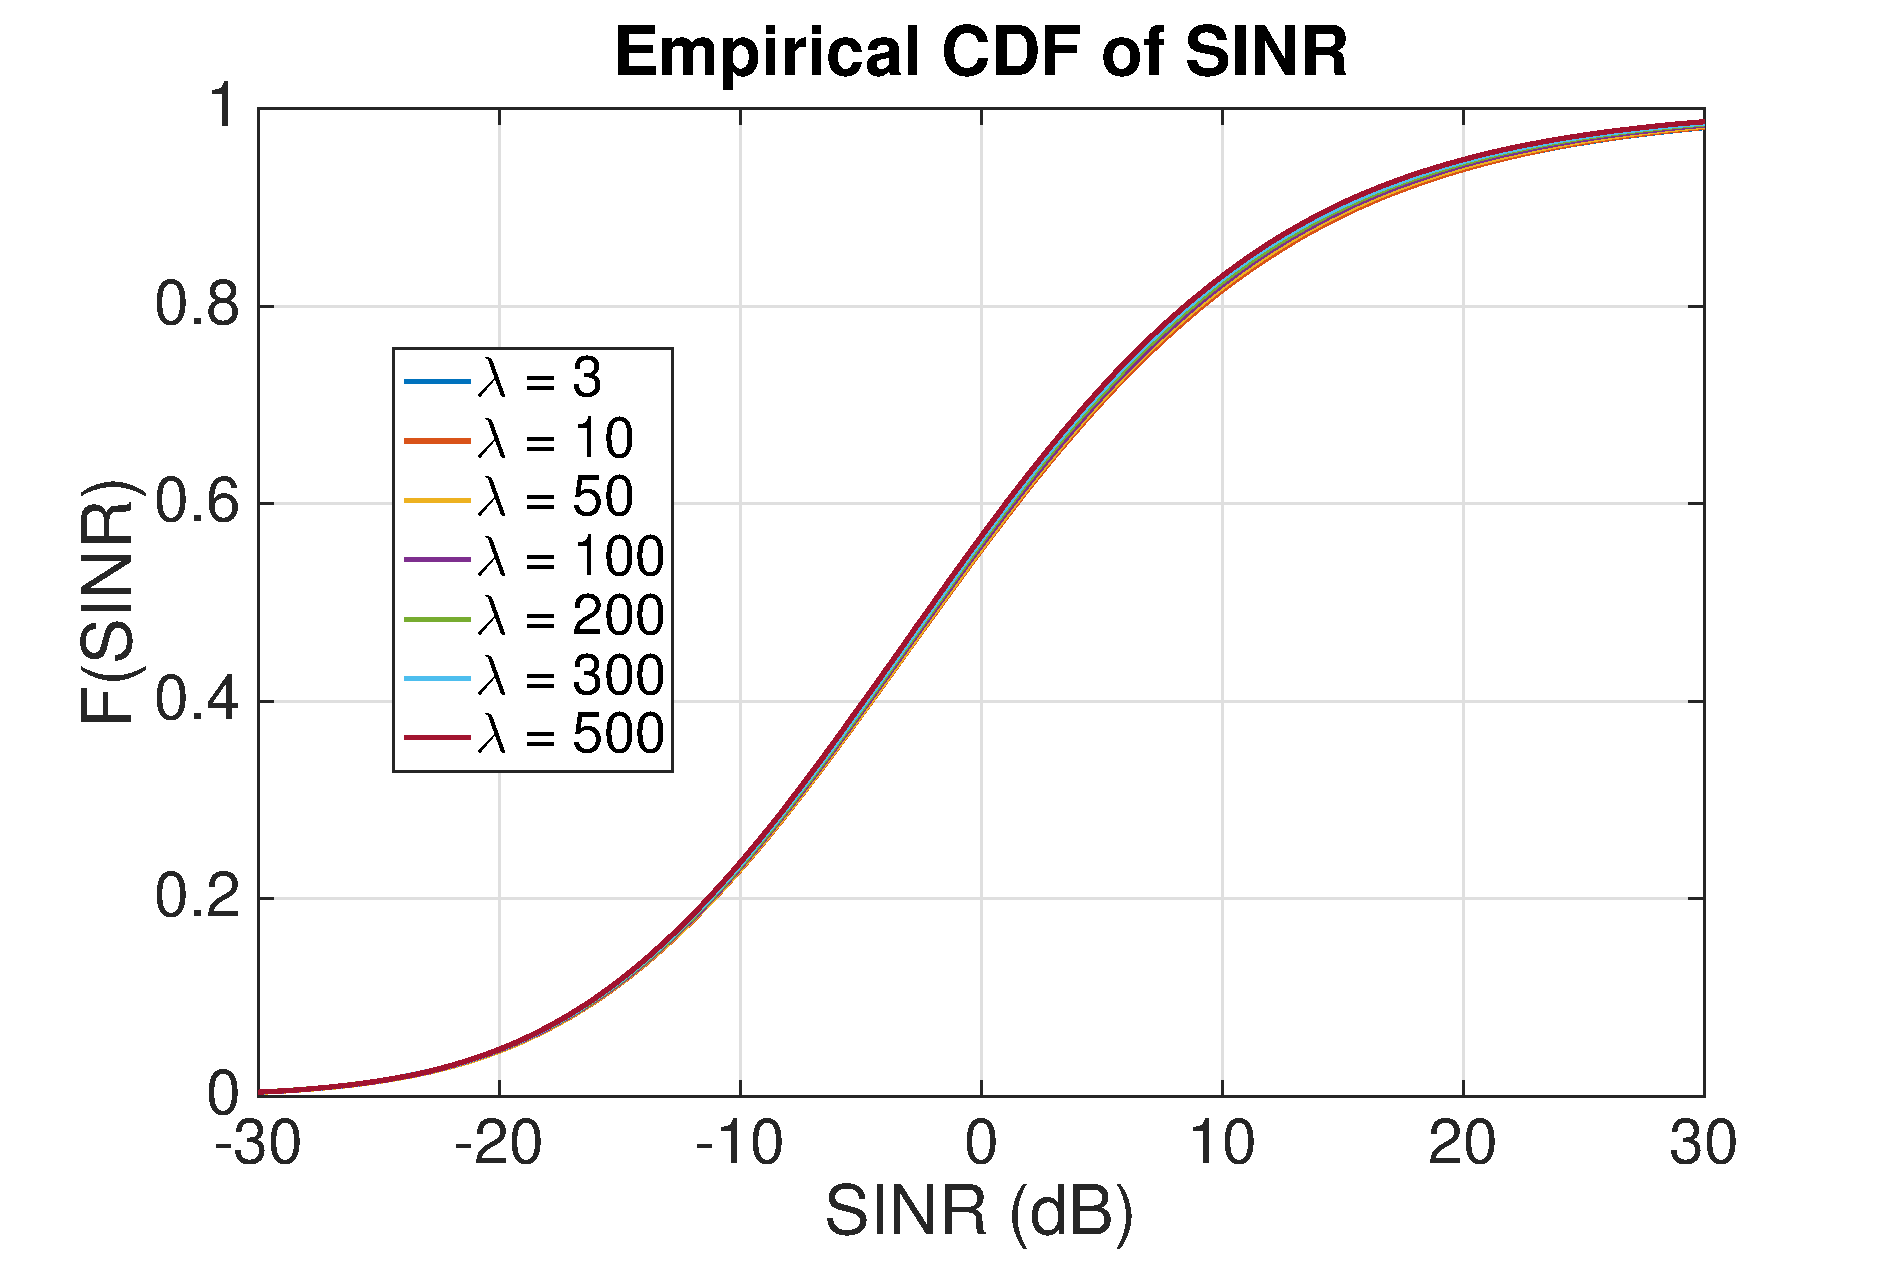
\includegraphics[width=5.5cm]{NBMax1000OutageProbCDFiid.eps}
\label{Mode1}}
\hfil
\subfigure[De-Correlation Distance: 20m]{
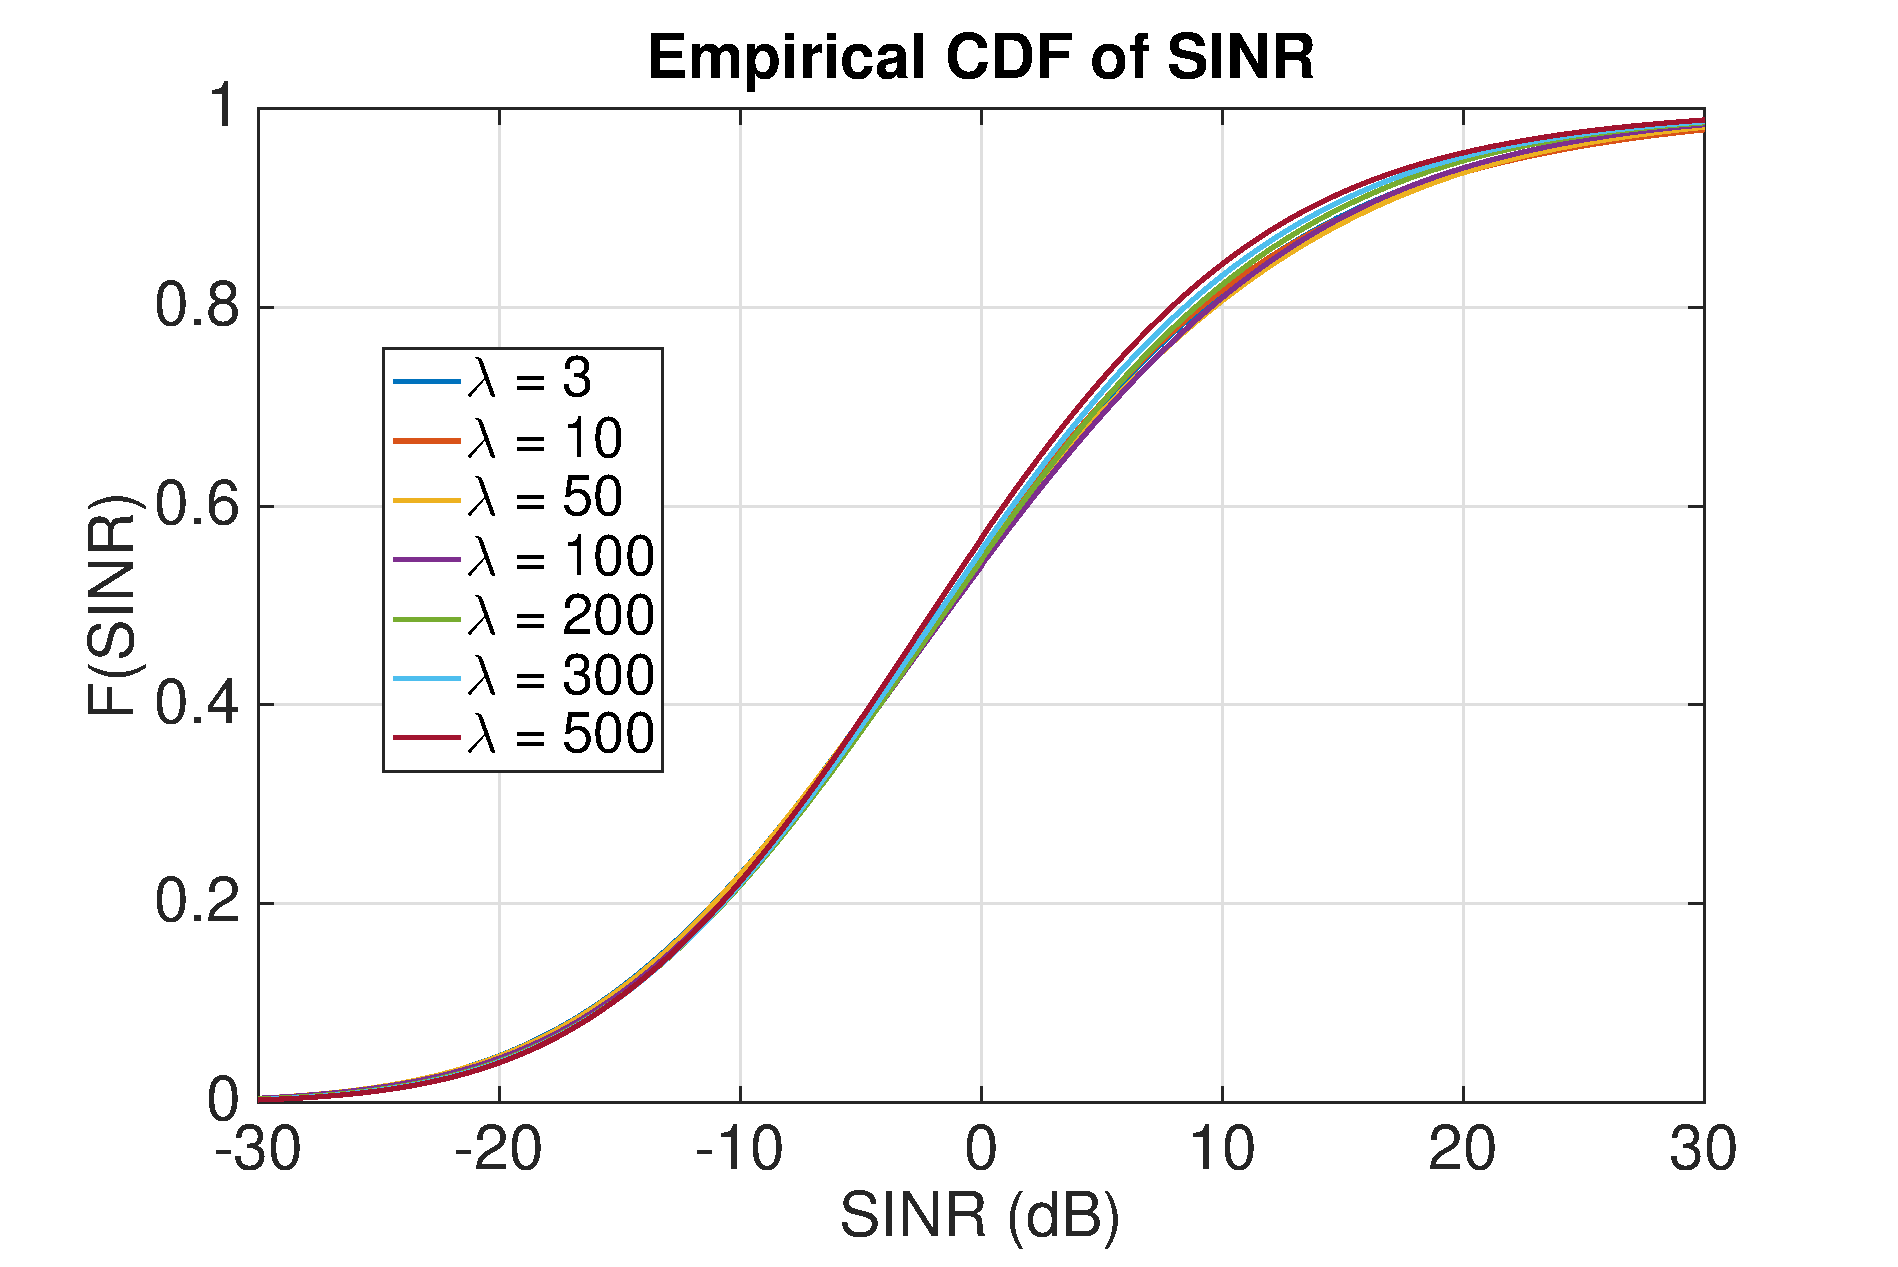
\includegraphics[width=5.5cm]{NBMax1000OutageProbCDFDeCorr20.eps}
\label{Mode2}}
\hfil
\subfigure[De-Correlation Distance: 200m]{
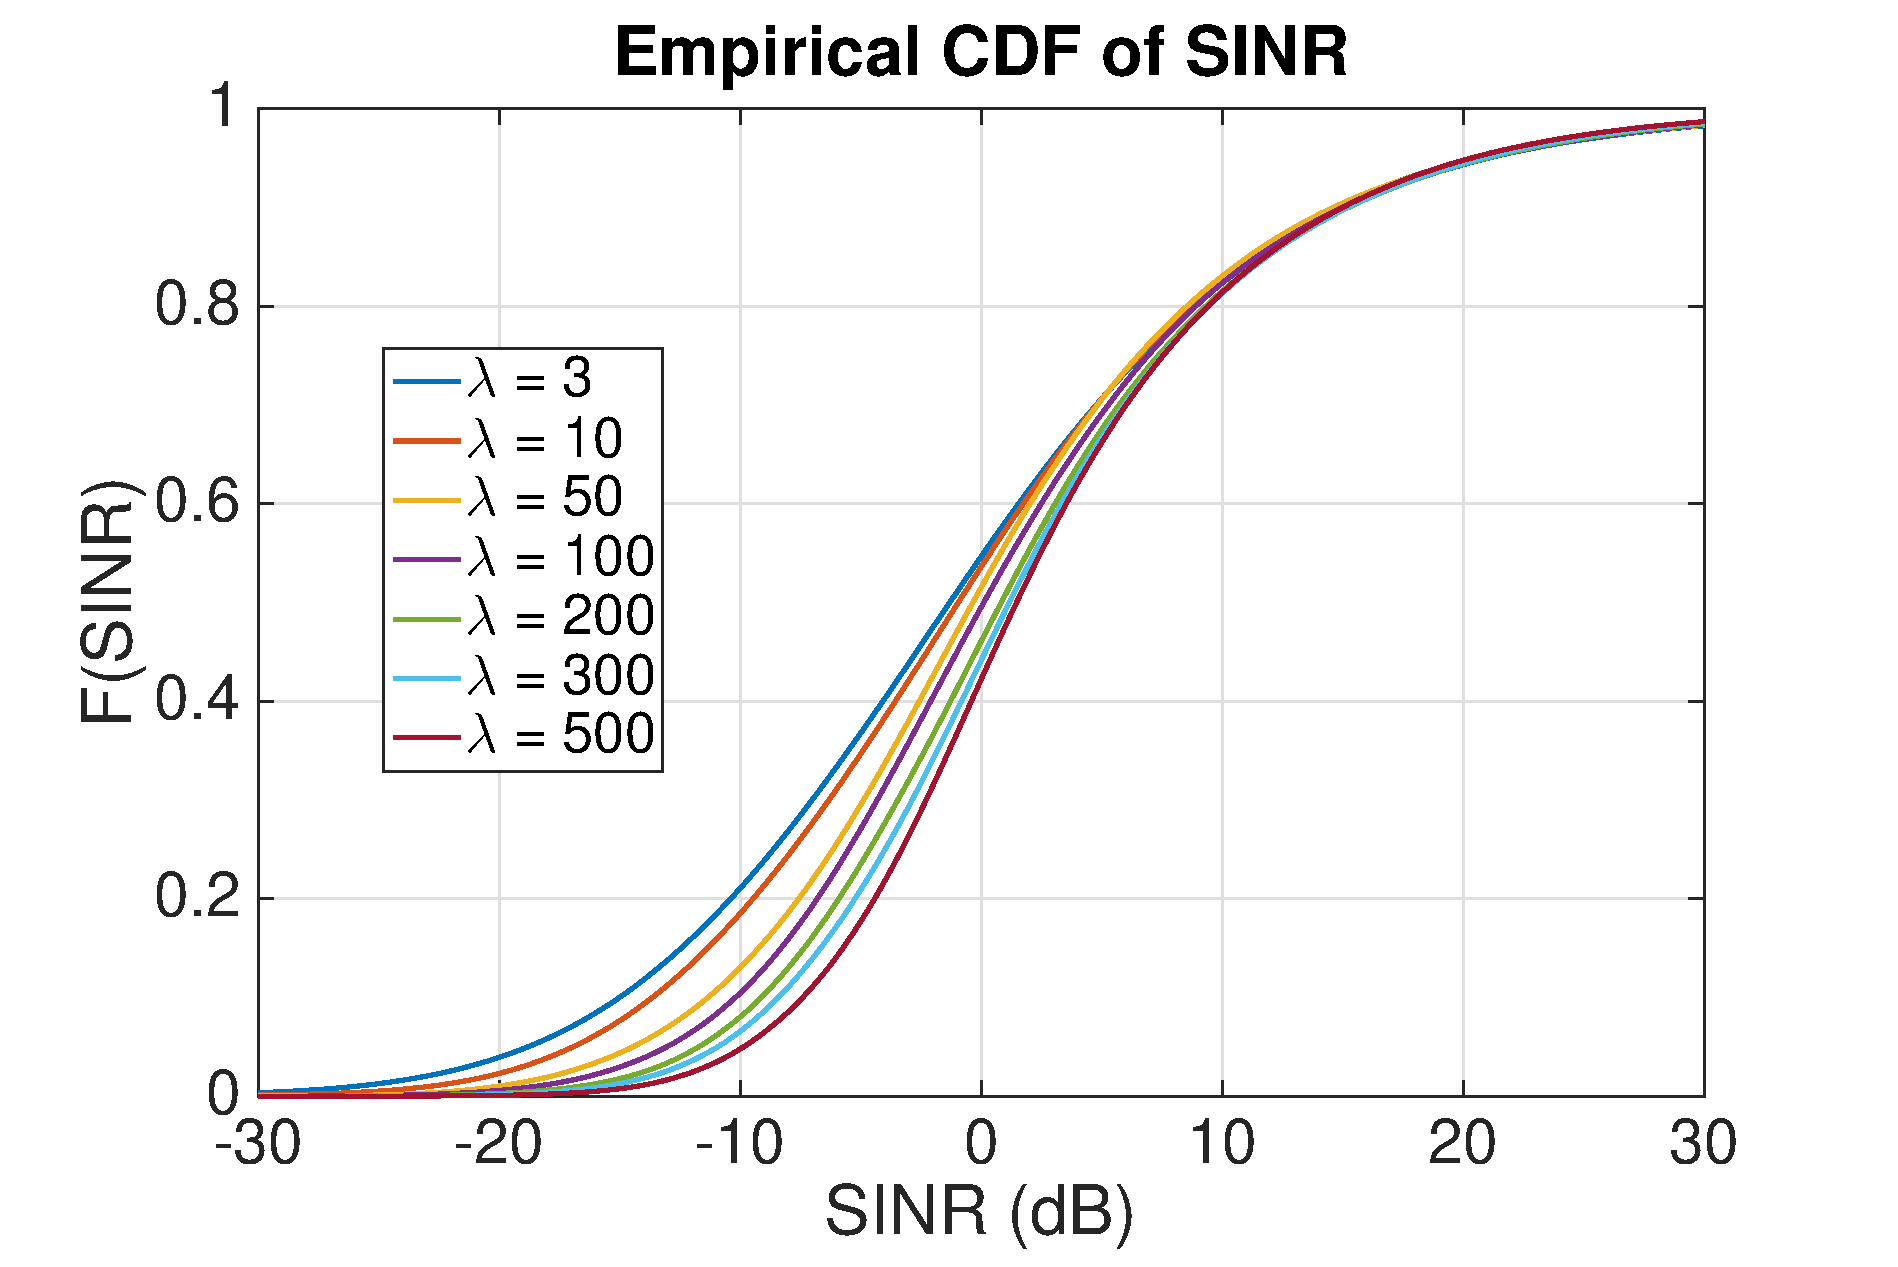
\includegraphics[width=5.5cm]{NBMax1000OutageProbCDFDeCorr200.eps}
\label{Mode3}}
\caption{CDF of SINR of MU when connecting to the nearest BS. (corresponding to three different shadow fading modes and several different BS densities.}
\label{nearestBS}
\end{figure*}
\begin{figure*}
\centering
\subfigure[i.i.d. Shadow Fading]{
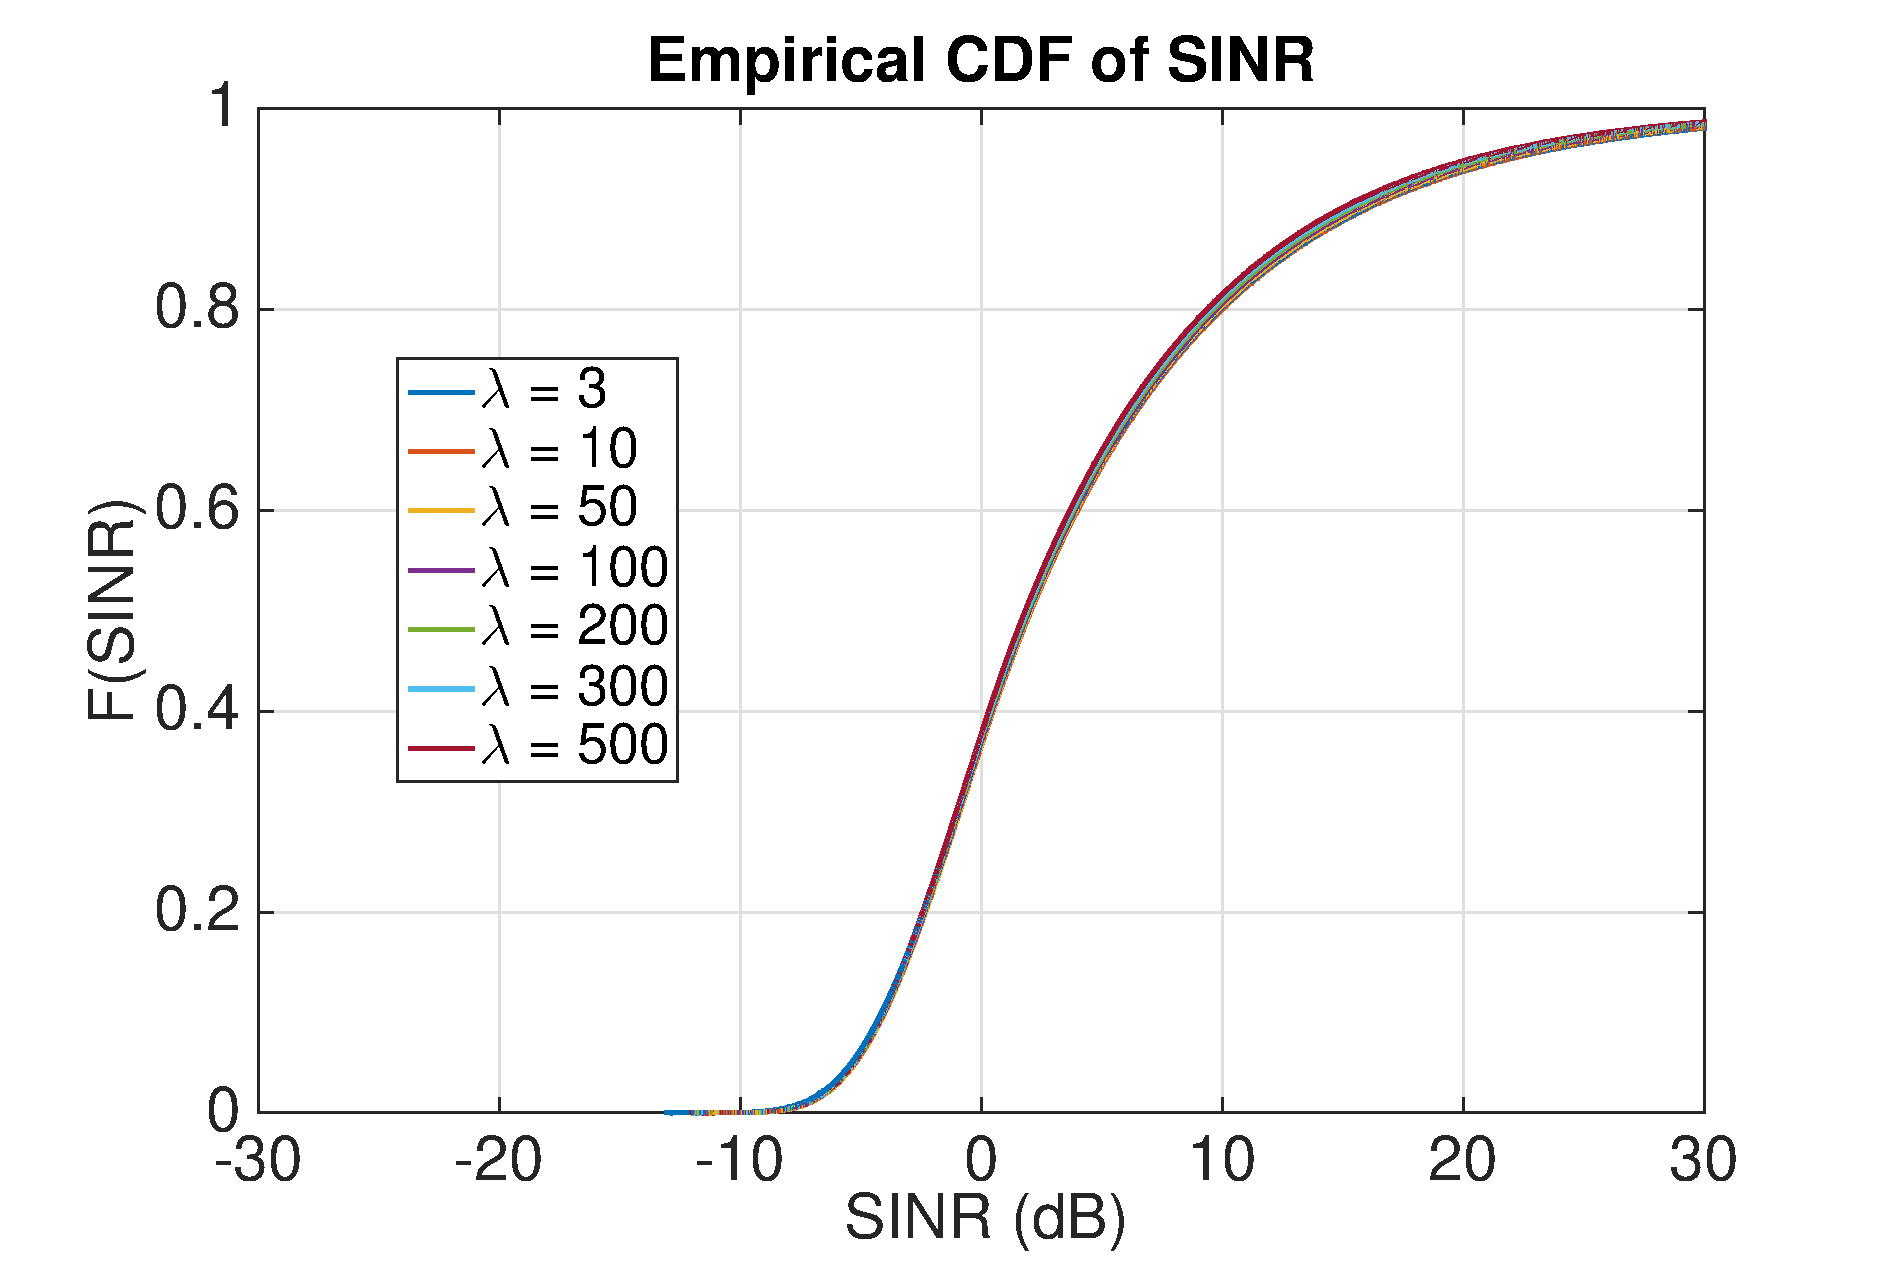
\includegraphics[width=5.5cm]{MaxMax1000OutageProbCDFiid.eps}
\label{Mode12}}
\hfil
\subfigure[De-Correlation Distance: 20m]{
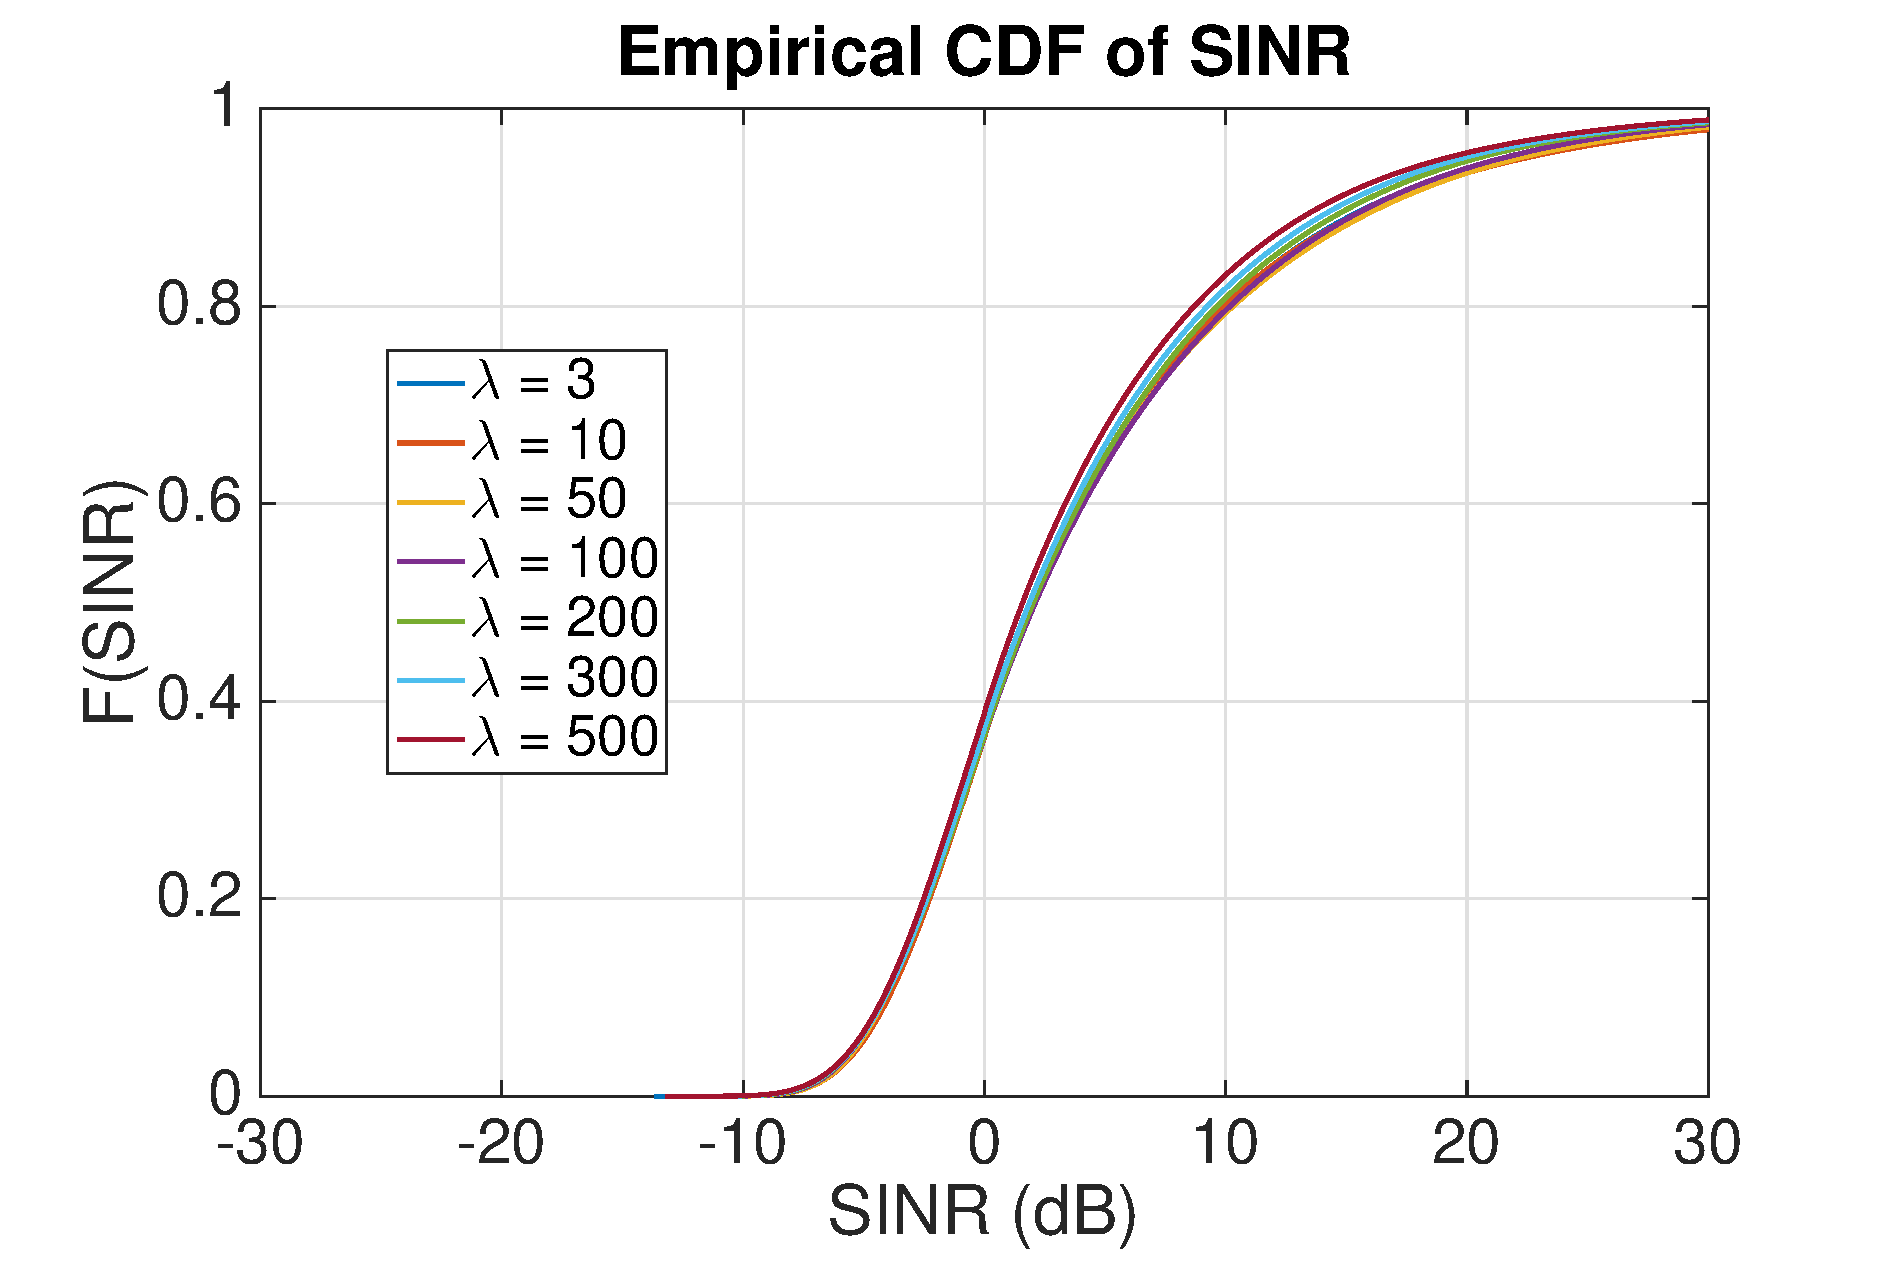
\includegraphics[width=5.5cm]{MaxMax1000OutageProbCDFDeCorr20.eps}
\label{Mode22}}
\hfil
\subfigure[De-Correlation Distance: 200m]{
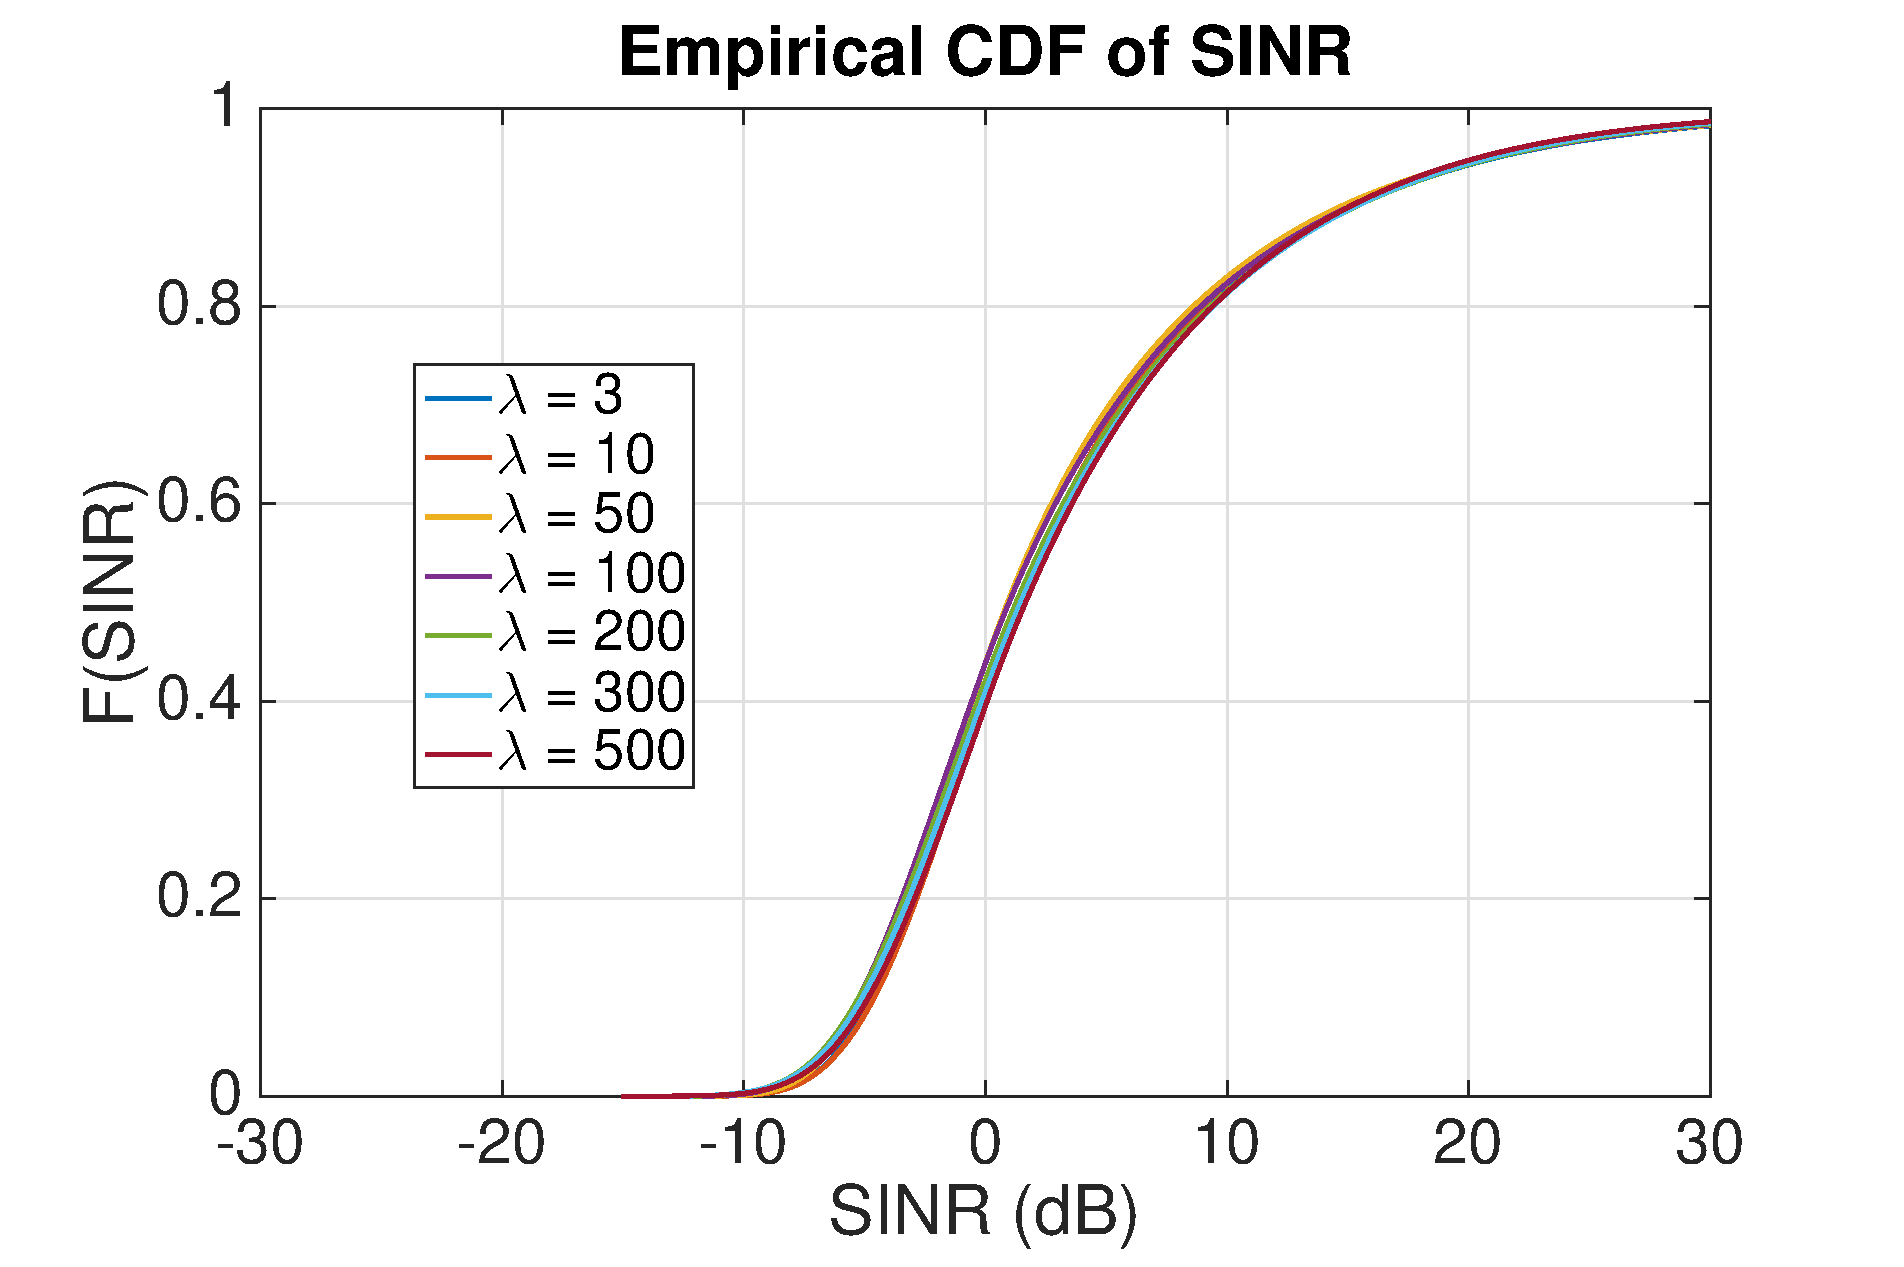
\includegraphics[width=5.5cm]{MaxMax1000OutageProbCDFDeCorr200.eps}
\label{Mode32}}
\caption{CDF of SINR of MU when connecting to the strongest BS. (corresponding to three different shadow fading modes and several different BS densities.}
\label{strongestBS}
\end{figure*}

In this section, we will present simulation setup and results. First, we run simulations to compare the outage probability of the two different network topology: Grid Layout and Random Layout. Secondly, SINR distribution and outage probability of Random Layout given different BS densities are investigated. Two scenarios are considered: MU connecting to the nearest BS and MU connecting to the BS providing strongest signal. At the end, the outage duration distribution are simulated and discussed given different BS densities. The values of parameters that are used in the simulation are shown in Table \ref{SystemConfig2}. 
\begin{table}
\centering
\caption{\label{SystemConfig2}Simulation Configuration Parameters}

\begin{tabular}{|c|c|}

\hline
Study Area & $1000m\times 1000m$\\
\hline
BS Densities & $3, 10,$\\
\hline
Pathloss Exponent & $4$\\
\hline
BS Transmission Power & $P: 40dbm$\\
\hline
SNR Requirement & $-5dB$\\
\hline
De-Correlation Distance & $20m, 200m$\\
\hline
\end{tabular}

\end{table}
\par Figure \ref{cdf1} shows the Cumulative Distribution Function (CDF) of SINR when MU connecting to the nearest BS. The de-correlation distance of the correlated shadow fading is $20m$. The figure suggests that Grid Layout outperforms the Random Layout, which is consistent with findings in \cite{andrews2011tractable}. Figure \ref{outage1} shows the outage probability with SINR threshold $-5dB$. The outage probability of Grid Layout (blue) is lower than the Random Layout (yellow). In next section, we will focus on the Random Layout which is more realistic than Grid Layout.


\par For Random Layout, SINR distribution and outage probability of different BS densities are investigated for both nearest BS connection and best channel BS connection. Simulations are run for \emph{i.i.d.} shadow fading and correlated shadow fading. CDF of SINR are calculated and outage probability given SINR threshold $-5dB$ are presented for increasing BS densities. Figure. \ref{nearestBS} shows the SINR of MU when connecting to the nearest BS. From Figure. \subref{Mode1} and \subref{Mode2} we can see that the CDF are overlapping each other which means increasing BS density does not change the CDF of SINR. From this we can conclude that when the shadow fading is \emph{i.i.d.} or the De-Correlation distance of the correlated shadow fading is small, increasing BS will not improve the system performance in terms of outage probability. Figure. \subref{Mode3}  shows that when increasing BS density, CDF of SINR improves (moves to the bottom-right corner). This suggests that when De-Correlation Distance is large, increasing BS density will result in better system performance in terms of outage probability. Figure. \ref{fig: outprob1} shows the outage probability of different correlated shadow fading models and different BS densities when SINR threshold is set to $-5dB$. Blue and green bars suggest that increasing BS density will not decrease outage probability when shadow fading is \emph{i.i.d} or shadow fading has $20m$ De-Correlation distance. Yellow bars suggest that when the De-correlation distance is $200m$, increasing BS density will decrease outage probability. For example, when BS is $3$, the outage probability is around $0.38$. Increasing BS density to $500$, the outage probability is decreased to $0.18$. From all above simulation results, we conclude that when De-Correlation distance is relatively large and MU is connecting to the nearest BS, increasing BS density will improve system performance in terms of decreasing outage probability.



\begin{figure}
\centering
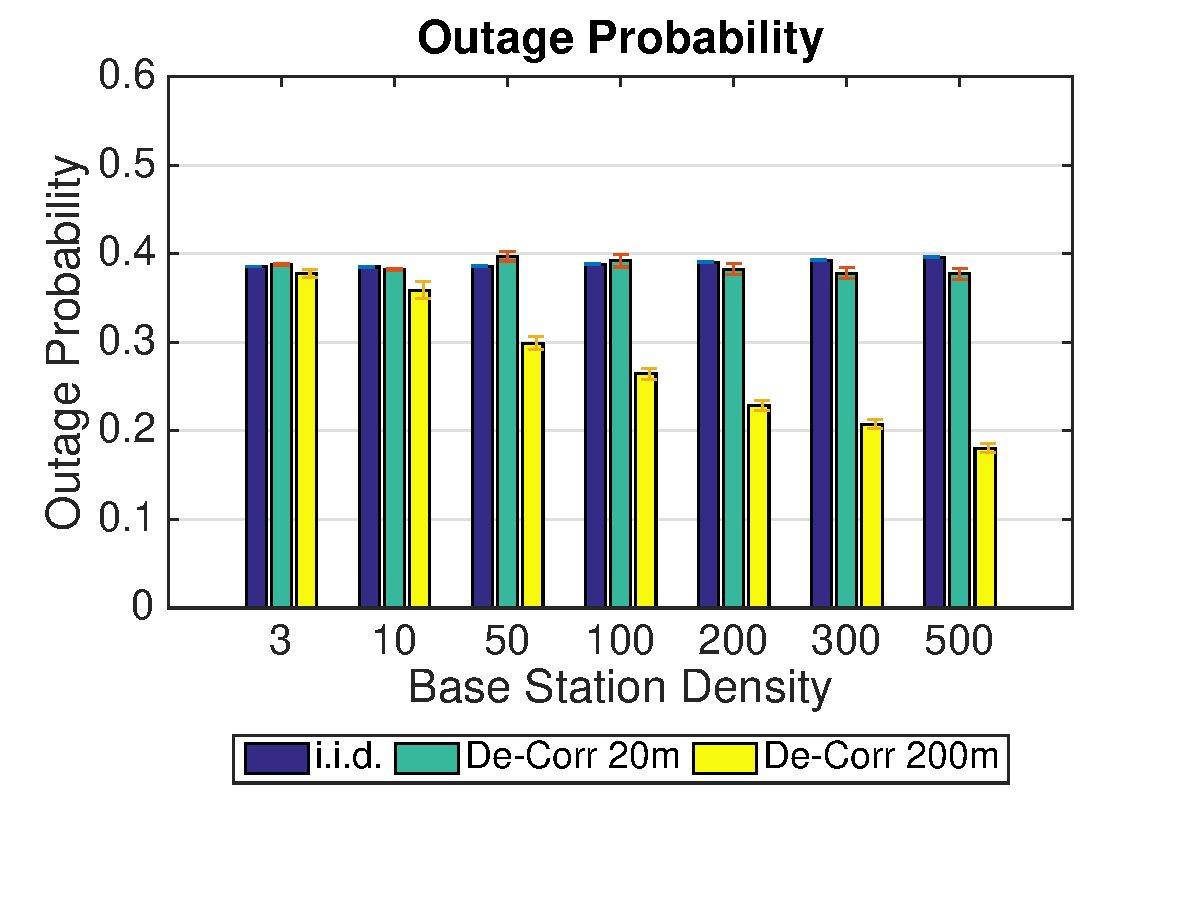
\includegraphics[width=6cm]{NBMax1000OutageProbThresh-5iid.eps}
\caption{Outage probability given SINR threshold to be $-5dB$}
\label{fig: outprob1}
\end{figure}
\begin{figure}
\centering
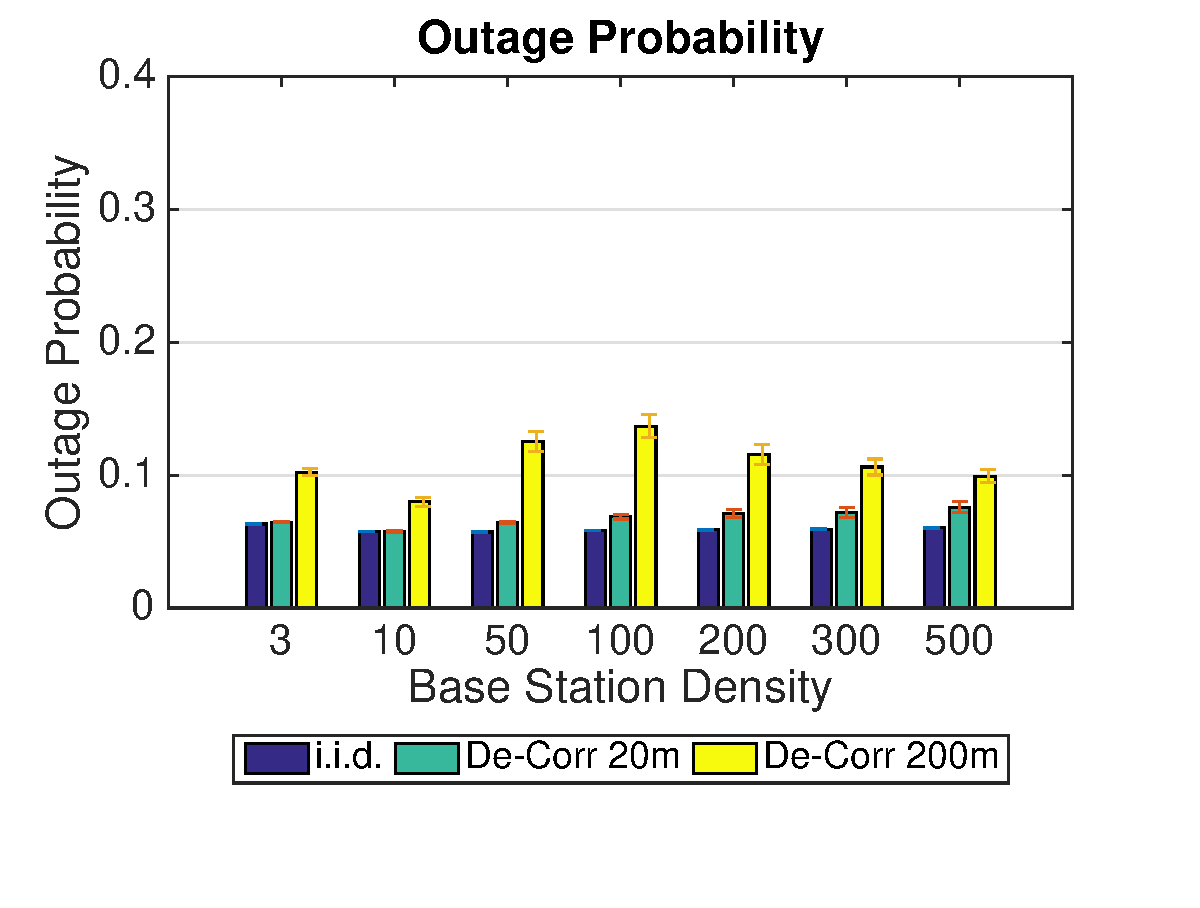
\includegraphics[width=6cm]{MaxMax1000OutageProbThresh-5iid.eps}
\caption{Outage probability given SINR threshold to be $-5dB$}
\label{fig: outprobs2}
\end{figure}
\begin{figure*}
\centering
\subfigure[Nearest BS with i.i.d. shadowing]{
\includegraphics[width=3.5cm]{ODthresh-5iidNB.eps}
\label{iid1}}
\hfil
\subfigure[Strongest BS with i.i.d. shadowing]{
\includegraphics[width=3.5cm]{ODthresh-5iidMax.eps}
\label{iid2}}
\hfil
\subfigure[Nearest BS with correlated shadowing (De-Correlation distance: 200m)]{
\includegraphics[width=3.5cm]{ODthresh-5DeCorr200NB.eps}
\label{corr1}}
\hfil
\subfigure[Strongest BS with correlated shadowing (De-Correlation distance: 200m)]{
\includegraphics[width=3.5cm]{ODthresh-5DeCorr200Max.eps}
\label{corr2}}
\caption{CDF of Outage Duration of MU when connecting to the nearest and strongest BS with i.i.d. shadow fading or correlated shadow fading}
\label{NBOD}
\end{figure*}
\par Next we move forward to investigate the system performance when the MU choose to connect to the BS which provides the strongest signal. Same simulations as the nearest BS scenario are run to study this scenario. Figure. \ref{strongestBS} shows the SINR of MU when connecting to the strongest BS. From subfigure \subref{Mode12}, \subref{Mode22} and \subref{Mode32} we can see that CDF of SINR almost overlap each other when increasing BS densities. This indicates that increasing BS density will not change CDF of SINR too much. Figure. \ref{fig: outprobs2} shows outage probability result which is consistent with our aforementioned conclusion. For each shadow fading model, the difference of highest outage probability and lowest outage probability is less than $0.5$. Compare three different shadow fading models, we can conclude that when the MU is connecting to the strongest BS, long De-Correlation distance will harm the system performance in terms of outage probability (yellow bars are higher than green or blue bars). 
\par Comparing Figure. \ref{fig: outprob1} and Figure. \ref{fig: outprobs2}, we can see that with same BS density, when MU connecting to the strongest channel, the outage probabilities are lower for every shadow fading model. For example, with \emph{i.i.d.} shadow fading and BS density to be $50$, the outage probability of connecting to nearest BS is $0.38$ while that of connecting to strongest BS is $0.06$. For correlated shadow fading with De-Correlation distance being $200m$, take the BS density $50$ as an example, we found that the outage probability of connecting to nearest BS is around $0.3$, which is higher than that of connecting to strongest BS, which is $0.14$. This suggests given the same network setup, connecting to the BS which provides strongest channel will improve the system performance. 








\par Next, we will investigate the system performance in terms of outage duration. We use Random Waypoint mobility model to model the user mobility. The parameters of the Random WayPoint model is given as in Table. \ref{RWP}. The MU speed is assume to be between $1m/s$ (pedestrian speed) to $20m/s$ (high way car speed). The MU pause interval is assumed to be uniformly between $0s$ to $60s$. The simulation time is set to be $0.1s$, which means for every $0.1s$ we check the MU's SINR to determine if it is still in the outage area or not.  The simulation result is showed in Figure. \ref{NBOD}. Comparing Figure. \subref{iid1} and Figure. \subref{corr1}, Figure. \subref{iid2} and Figure. \subref{corr2}, we can see that when the channel is experiencing i.i.d. shadow fading, the outage duration is usually less than $2s$. However,  when the channel is under correlated shadow fading with De-Correlation distance equal to $200m$, the outage duration can be longer than $30s$. Therefore, we can conclude that correlated shadow fading brings long outage duration to the system. Comparing Figure. \subref{iid1} and Figure. \subref{iid2}, we found that with i.i.d. shadow fading, connecting to strongest BS will reduce the outage duration.  Nevertheless, Figure. \subref{corr1} and Figure. \ref{corr2} suggests that changing connection strategy will not improve the outage duration in terms of distribution, although connecting to strongest BS will reduce outage probability. Both Figure. \subref{corr1} and Figure. \subref{corr2} indicate that increasing BS density will reduce long outage duration. For example, in Figure. \subref{corr1}, when the BS density increase from $50$ to $300$, the probability of outage duration longer than $10s$ is reduced from $24\%$ to $7\%$. In contrast, for i.i.d. shadow fading, increase BS density will not change the distribution of outage duration, which is confirmed by Figure. \ref{iid1} and Figure. \ref{iid2}. All CDF curve of outage duration overlap each other when BS density changes. 
\begin{table}
\centering
\caption{\label{RWP}Random Waypoint Mobility Model Parameters}

\begin{tabular}{|c|c|}

\hline
Speed Interval & $1 - 20m/s$\\
\hline
Pause Interval & $0 - 60s$\\
\hline
Simulation Time & $0.1s$\\
\hline
\end{tabular}

\end{table}

\section{Conclusions}
\label{Conclusion}
Shadow fading is large-scale fading which can cause significant received power loss for a wide area. In general, shadow fading is considered to be i.i.d. to simplify the analysis. However, this is not the real case. In reality, shadow fading at two different positions are correlated to each other. Correlated shadow fading will result in correlated long outage durations. Power outage will lead to connection loss and/or packet loss which is harmful to MUs, especially to those who are using real-time applications such as video conferencing. To investigate a multi-cell system performance given correlated shadow fading, simulations are run to study the outage probability and outage duration distribution. First of all, the probability of two different BS layout: Grid Layout and Random Layout are investigated. We found that Grid Layout performs better than Random Layout. Secondly, outage probability given different BS densities and two different connecting strategies: nearest BS and strongest BS, are simulated. We conclude that connecting to strongest BS will reduce the outage probability comparing with nearest BS. Increasing BS density will not reduce outage probability when MU is connecting to the strongest BS. However, when MU is connecting to the nearest BS and the De-Correlation distance of correlated shadow fading is large enough, increasing BS density will reduce the outage probability, therefore improve the system performance. At last, we investigate system performance in terms of outage duration. The simulation results show that correlated shadow fading will result in long outage duration. Increasing BS density will efficiently reduce the percentage of long outage duration.



\bibliography{mybib}

\begin{IEEEbiography}{Michael Shell}
Biography text here.
\end{IEEEbiography}

% if you will not have a photo at all:
\begin{IEEEbiographynophoto}{John Doe}
Biography text here.
\end{IEEEbiographynophoto}

% insert where needed to balance the two columns on the last page with
% biographies
%\newpage

\begin{IEEEbiographynophoto}{Jane Doe}
Biography text here.
\end{IEEEbiographynophoto}
\end{document}